\documentclass[a4paper,11pt]{report}

\usepackage[T1]{fontenc}
\usepackage[utf8]{inputenc}
\usepackage[italian]{babel}

\usepackage{mathdots}
\usepackage{mathtools}
\usepackage{graphicx}
\usepackage{amsfonts}
\usepackage{amsthm}
\usepackage{amsmath}
\usepackage{amssymb}
\usepackage{fancyhdr}
\usepackage{float}
\usepackage{geometry}
\geometry{a4paper, top=2.5cm, bottom=2cm, left=2cm, right=2cm}
\usepackage{hyperref}
\hypersetup{
	colorlinks=true,
	linkcolor=blue,
	filecolor=blue,
	citecolor = black,      
	urlcolor=cyan,
}

\swapnumbers
\theoremstyle{remark}
\newtheorem*{oss}{Oss}
\newtheorem*{nb}{N.B}
\newtheorem*{coro}{Corollario}
\theoremstyle{definition}
\newtheorem*{teo}{Teorema}
\newtheorem*{Def}{Def}

\newcommand{\C}{\mathbb{C}}
\newcommand{\R}{\mathbb{R}}

\DeclarePairedDelimiter{\abs}{\lvert}{\rvert}

\begin{document}
	\date{}
	\author{Marco Militello}
	\title{Matematica per la fisica}
	\maketitle
	\tableofcontents
	\newpage
	
\part{Analisi complessa}

\chapter{Numeri complessi}
\begin{Def}
	Un numero complesso è una coppia ordinata $(a,b)$ con $a,b \in \R$ tale che siano definite
	\begin{center}
	\begin{tabular}{ll}
		 Addizione  & $[(a,b)+(c,d) = (a+c, b+d)]$\\
		 Moltiplicazione & $[(a,b)(c,d) = (ac-bd, ad+bd)]$ \\
		 Relazione di equivalenza & $[(a,b) = (c,d) \iff a=c \; b=d]$
	\end{tabular}
 	\end{center}
\end{Def}
\begin{teo}
	\[\C = \{(a,b)\, | \, a,b \in \R\}\]
	è un campo Abeliano rispetto addizione e moltiplicazione
\end{teo}
\begin{oss}\hfil
	\begin{itemize}
		\item Proprietà commutativa e associativa seguono da quelle dei reali
		\item Identità additiva \quad $(0) \rightarrow (0,0)$
		\item Esiste opposto: \quad $(a,b) + (-a,-b) = (0,0)$
		\item Identità moltiplicativa: \quad $(1) \rightarrow (1,0)$
		\item Esiste inverso: \quad $(a,b)\frac{1}{(a,b)}= (1,0) \; \frac{1}{(a,b)} = \left(\frac{a}{a^2+b^2}, -\frac{b}{a^2+b^2}\right)$
	\end{itemize}
\end{oss}
\begin{teo}\hfill\\
	Il sottoinsieme $\C_0 = \{(a,0) \, | \, a \in \R\} \subset \C$ è un campo rispetto ad addizione e moltiplicazione \newline
	$\C_0$ è ISOMORFO a $\R$
\end{teo}
\begin{Def}{\textbf{Unità immaginaria}}
	\[(0,1) = i\]
	$(0,1)(0,1) = (-1,0) \qquad (0,-1)=-i$
\end{Def}
\begin{Def}[\textbf{Forma cartesiana}]
	\[z = (a,b) = a + ib \qquad a,b \in \R; \, z \in \C\]
	$a = Re\{z\} \quad b=Im\{z\}$
\end{Def}
\begin{Def}[\textbf{Coniugazione complessa}]
	\[\bar{z} = a-ib = (a,-b) \quad z = a+ib = (a,b)\]
\end{Def}
Operazioni notevoli:
\begin{itemize}
	\item $z + \bar{z} = 2Re\{z\} = 2a$
	\item $z-\bar{z} = 2iIm\{z\} = 2ib$
	\item  $z\bar{z} = a^2+b^2 = \abs{z}^2$
\end{itemize}

\section{Piano complesso (Armand-Gauss)}
\begin{figure}
	\centering
	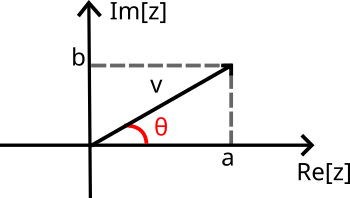
\includegraphics[width=0.4\linewidth]{immagini/piano_gauss}
\end{figure}
\begin{gather*}
	\abs{\vec{v}} = \abs{z} = \sqrt{a^2+b^2} \\
	\begin{cases}
		a = \abs{z}\cos\theta \\
		b = \abs{z}\sin\theta
	\end{cases}
\end{gather*}
Somma come somma vettoriale
\begin{Def}[\textbf{Coordinate polari}]
	\[z = a+ib = r(\cos\theta + i \sin\theta) \quad r= \sqrt{a^+b^2} \quad \tan\theta = \frac{b}{a}\]
	\[\arg(z)=\theta=
	\begin{cases}
		\arctan\left(\frac{b}{a}\right) & a>0 \\
		\arctan\left(\frac{b}{a}\right) + \pi & a<0 \; b>0 \\
		\arctan\left(\frac{b}{a}\right) -\pi & a<0 \; b<0 \\
		\frac{\pi}{2} & a=0 \; b>0 \\
		-\frac{\pi}{2} & a=0 \; b<0
	\end{cases}\]
\end{Def}
\subsection*{Formula di Eulero}
Estendere $e^\gamma \quad \text{con } \gamma \in \R$ \; a \; $e^z \quad \text{con } z \in \C$ 
\[e^z = e^x(\cos(y)+i\sin(y))\]
\begin{oss}
	\begin{gather*}
		z = re^{i\theta} \rightarrow \bar{z} = re^{-i\theta} \\
		z_1z_2 = r_1r_2e^{i(\theta_1 + \theta_2)}
	\end{gather*}
\end{oss}
\subsection*{Formula di De Moivre}
Se $n \in \mathbb{Z} $ si ha:
\[z^n = r^n(\cos(n\theta) +i \sin(n\theta))\]
\subsection*{Radice n-esima}
Se $n \in \mathbb{Z}$ si ha:
\[z^{\frac{1}{n}} = \sqrt[n]{r} \left(\cos\left(\frac{\theta + 2k\pi}{n}\right) + i\sin\left(\frac{\theta + 2k\pi}{n}\right)\right)\]
Allora esistono n diverse radici si $z$ se $\abs{z} \neq 0$
\subsection*{Equazioni di secondo grado in $\C$}
\[az^2+bz+c \qquad \text{con } a,b,c \in \R \; z \in \C\]
Ha sempre 2 soluzioni 
\begin{itemize}
	\item[*] Se $\Delta = b^2 - 4ac \geq 0 \; \Rightarrow$ 2 soluzioni reali
	\item[*] Se $\Delta <0 \; \Rightarrow -\Delta >0 \Rightarrow z_{1,2} \in \C \text{ e } z_1 = \bar{z}_2$
\end{itemize}
\subsection*{Logaritmo}
\[\log(z) = \log(r) + i\phi\]
Così definito il logaritmo è una funzione palindroma, cioè assume valori differenti a seconda $\theta \mapsto \theta + 2k\pi$
Allora scelgo $\theta$ per aver $\log(z)$ univoco
\[\theta \in
\begin{cases}
	[0,\pi] & y>0 \\
	[-\pi,0] & y<0
\end{cases}\]
\begin{nb}
	$\log(z)$ è discontinuo per $x \in (-\infty,0]$ \newline
	Allora escludo $(-\infty,0] \Rightarrow \C \smallsetminus (-\infty,0) \Rightarrow$ BRANCH CUT
\end{nb}
\noindent Definiamo 
\[\log(z) = \log(r) +i\arg(z)\]
$\overline{\log(z)} = \log(\bar{z})$
\subsection*{Norma}
Su $\C$ è definita la norma $\abs{z}$ che soddisfa le proprietà di una distanza $d(a,b) \quad a,b \in \C$
\begin{itemize}
	\item $d(a,b) = d(b,a)$
	\item $d(a,b) = 0 \iff a=b$
	\item $\forall c \in \C \Rightarrow d(a,b) + d(b,c) \geq d(a,c)$
\end{itemize}
\noindent \'E possibile allora definire la distanza 
\[d(z_1,z_2) = \abs{z_1-z_2} \qquad z_1,z_2 \in \C \]
\begin{Def}[\textbf{Successione di Cauchy}]\hfill\\ \label{cauchy}
	\[\{z_k\} \; \text{tale che} \; \forall \epsilon>0 \; \exists N_\epsilon>0 \; | \; \forall n,m>N_\epsilon \Rightarrow \abs{z_n-z_m}<\epsilon\]
\end{Def}
\begin{nb}\hfill
	\begin{enumerate}
		\item $\{z_k\}$ è di \hyperref[cauchy]{Cauchy} se lo sono anche $\{Re(z_k)\} \text{ e } \{Im(z_k)\}$ 
		\item Tutte le successioni convergenti sono di \hyperref[cauchy]{Cauchy}; in $\C$ è vero anche il viceversa perchè $\C$ è completo
	\end{enumerate}
\end{nb}
\begin{Def}[\textbf{Serie su $\C$}]\hfil\\
	La serie $\sum_n z_n$ con $z_n \in \C$ converge a $z \in \C$ se la successione delle somme parziali $\{S_n\}$ converge a $z$
	\[S_n = \sum_{k=0}^{n-1} z_n\]
\end{Def}
\newpage
\begin{oss}\hfil
	\begin{itemize}
		\item Condizione necessaria convergenza: \quad $z_n \to 0 \text{ per } n \to \infty$
		cioè 
		$\begin{cases}
			Re(z_n) \to 0 \\
			Im(z_n) \to 0
		\end{cases}$
		\item Condizione sufficiente: CONVERGENZA ASSOLUTA cioè \newline
		Se converge $\sum \abs{z_n}$  su $\R \Rightarrow$ converge anche $\sum z_n$ su $\C$
	\end{itemize}
\end{oss}
\begin{Def}
	\[e^{i\theta} = \sum_{n=0}^{\infty} \frac{1}{n!} {(i\theta)}^n\]
\end{Def}
\begin{oss}
	$e^{i\theta} = \cos\theta + i\sin\theta$
\end{oss}
\begin{Def}[\textbf{Serie di potenze}]\hfil\\
	$S(z,z_0)$ con $z,z_0 \in \C \text{ e } z_0$ centro si ha:
	\[S(z,z_0) = \sum_{n=0}^{\infty} a_n {(z-z_0)}^n \quad an=cost \, \in \C\]
\end{Def}
\noindent Convergenza per ogni $z$ fissato $\Rightarrow$ 	CONVERGENZA PUNTALE
\begin{oss}
	\[E = \{z \in \C \; | \; S(z,z_0) \text{ è convergente}\}\]
	$E$ non è mai vuoto $\rightarrow z_0 \in E$ e $S(z,z_0) = a_0$ cioè converge 
\end{oss}
\begin{Def}[\textbf{Raggio di convergenza}] \label{def:raggio conv} 
	\[D = \{\abs{z-z_0} \; \forall z \in E\}\]
	Raggio di convergenza:
	\[R = \sup_{z \in E} D\]
	cioè la maggior distanza da $z_0$ per cui la serie converge
\end{Def}
\begin{oss}\hfil
	\begin{itemize}
		\item Le serie di potenze su $\C$ convergono in un cerchio di raggio $R$
		\item Se la serie converge solo in $z=z_0 \Rightarrow R=0$
		\item Se la serie converge $\forall z \in \C \Rightarrow R=\infty$
	\end{itemize}
\end{oss}
\subsubsection*{Calcolo del raggio di convergenza}
\begin{enumerate}
	\item $ \displaystyle R = {\left(\lim_{n \to \infty} \sup_{k \geq n} {\abs{a_k}}^\frac{1}{k}\right) }^{-1}$ \newline
	Si riduce a $\displaystyle \lim_{n \to \infty} \frac{1}{{\abs{a_n}}^{\frac{1}{n}}}$ se tale limite esiste
	\item  $\displaystyle R =\lim_{n \to \infty} \frac{\abs{a_n}}{\abs{a_{n+1}}}$ se tale limite esiste 
\end{enumerate}
\noindent Calcolato $R \Rightarrow$ 
$\begin{cases}
	\abs{z-z_0}<R & \text{la serie converge} \\
	\abs{z-z_0}>R & \text{la serie diverge} \\
	\abs{z-z_0}=R & \text{si studia caso per caso}
\end{cases}$
\begin{oss}
	La derivata di una serie di potenze con raggio di convergenza $R$ ha lo stesso raggio di convergenza
\end{oss}
\begin{coro}
	Una serie di potenze è infinitamente differenziabile all'interno del suo raggio di convergenza
\end{coro}
\chapter{Funzioni complesse}
\begin{Def}[\textbf{Funzione complessa}] \label{def:f complessa} \hfil\\
	Una funzione complessa è una mappa 
	\[f: \, \C \to \C \]
	che associa un punto $z \in \C$ a un punto $w = f(z) \in \C$
	\[f(z) = Re(f(z)) + iIm(f(z)) \Rightarrow f(z) = u(x,y) + iv(x,y)\]
	$u,v$ funzioni su $\R^2$ di $x,y \in \R$
\end{Def}
\begin{Def}[\textbf{Continuità}] \label{def:continuità} \hfill\\
	$f(z)$ è continua in $z_0 \in \C$ se è definita in un intorno di $z_0$ ed esiste finito il limite 
	\[\lim_{z \to z_0} f(z) = f(z_0)\]
\end{Def}
\begin{Def}[\textbf{Limite}]\label{def:limite}\hfil\\
	$f(z_0)$ è il limite di $f(z)$ per $z \to z_0$ se:
	\[\forall \epsilon>0 \; \exists \delta>0 \; | \; \abs{z-z_0}<\delta \text{ se } \abs{f(z)-f(z_0)}<\epsilon\]
\end{Def}
\begin{nb}
	Come per $\R^2$ il limite deve essere indipendente dal cammino
\end{nb}
\begin{Def}[\textbf{Continuità su un dominio}]\hfil\\
	$f(z)$ è continua su un $D \subseteq \C$ se è continua $\forall z \in D$
\end{Def}
\begin{Def}[\textbf{Derivata si una funzione continua}]\hfil\\
	$f(z)$ è differenziabile se esiste il limite
	\[\lim_{z \to z_0} \frac{f(z)-f(z_0)}{z-z_0} = f'(z_0) = \frac{df}{dz}\Bigr|_{z_0}\]
\end{Def}
\begin{nb}
	Anche la derivata è indipendente dal cammino
\end{nb}
\begin{Def}[\textbf{Funzione olomorfa}]\label{def:olomorfa}\hfil\\
	Una funzione differenziabile su $D \subseteq \C$ si dice OLOMORFA
\end{Def}
\subsubsection*{Proprietà funzioni olomorfe}
\begin{itemize}
	\item $(f \pm g)' (z) = f'(z) \pm g'(z)$
	\item $(fg)'(z) = f'(z)g(z) + f(z)g'(z)$
	\item $\left(\frac{f}{g}\right)'(z) = \frac{f'(z)g(z) - f(z)g'(z)}{g^2(z)} \quad g(z) \ne 0$ 
	\item Funzione composta: \quad $\frac{d}{dz} (f \circ g) (z) = f'(g(z))g'(z)$
	\item Derivata funzione inversa: data $w= f(z)$ olomorfa in $z_0$ con $f'(z_0)$ \newline
	$h(w) = z = f^{-1}(w) \text{ è olomorfa in } w_0=f(z_0) \text{ e } h'(w_0) = \frac{1}{f'(h(w_0))} = \frac{1}{f'(z_0)}$
\end{itemize}
\section{Condizioni di Cauchy-Riemann}
Condizioni necessarie e sufficienti per verificare differenziabilità
\begin{teo}\hfill\\
	$f(z) = u(x,y) + iv(x,y)$ tale che $u,v$ abbiano derivate parziali continue in un intorno di $z_0 = x_0 + iy_0$
	 \[\delta_x f(z_0) = i\delta_y f(z)\] cioè:
		\begin{itemize}
			\item $\delta_x u(x,y) \bigr|_{(x_0,y_0)} = \delta_y v(x,y) \bigr|_{x_0,y_0}$
			\item $\delta_y u(x,y) \bigr|_{(x_0,y_0)} = -\delta_x v(x,y) \bigr|_{x_0,y_0}$
		\end{itemize}
\end{teo}
\begin{oss}
	Le condizioni di Cauchy-Riemann permettono di scrivere le derivate complesse di $f(z) = u +iv$ in 4 modi equivalenti:
	\[f'(z) = \begin{cases}
		\delta_x u + i \delta_x v \\
		\delta_x u - i \delta_y v \\
		\delta_x u - i \delta_y u \\
		\delta_y u + i \delta_x u 
	\end{cases}\]
\end{oss}
\begin{Def}[\textbf{Operatori differenziali in $\bf {z,\bar{z}}$}]
	\begin{gather*}
		\delta_z = \frac{1}{2}(\delta_x - i\delta_y) \\
		\delta_{\bar{z}} = \frac{1}{2}(\delta_x + i\delta_y)
	\end{gather*}
\end{Def}
\begin{teo}\hfil\\
	Se $f(z)$ è olomorfa su un dominio $D \subseteq \C \Rightarrow \delta_{\bar{z}} f(z) =0$
\end{teo}
\begin{Def}[\textbf{Funzioni anti-olomorfe}]\hfil\\
	Una funzione si dice anti-olomorfa se
	\[\frac{\delta}{\delta z} f(z) =0\]
\end{Def}
\begin{oss}
	Si può dimostrare che se $f(z)$ è antiolomorfa $\Rightarrow \bar{f}(z)$ è olomorfa 
\end{oss}
\begin{Def}[\textbf{Funzioni trigonometriche}]
	\[\cos{z} = \frac{1}{2} (e^{iz} + e^{-iz}) \qquad \sin{z} = \frac{1}{2i} (e^{iz} - e^{-iz}) \]
\end{Def}
\begin{Def}[\textbf{Funzioni iperboliche}]
	\[\cosh{z} = \frac{1}{2} (e^z+e^{-z}) \qquad \sinh{z} = \frac{1}{2} (e^z-e^{-z})\]
\end{Def}
\section{Proiezione stereografica e punto all'infinito}
I numeri complessi sul piano $\C$ possono essere rappresentati come punti sulla superficie di una sfera
\[S^2 = \left\{(\xi,\eta,\zeta) \; \Bigr| \; \xi^2 + \eta^2 + {\left(\zeta - \frac{1}{2}\right)}^2 = \frac{1}{4}\right\}\]
\begin{figure}[H]
	\centering
	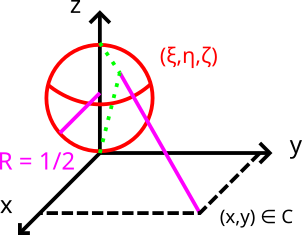
\includegraphics[width=0.6\linewidth]{immagini/sfera}
	\label{fig:sfera}
\end{figure}
\begin{gather*}
	x = \frac{\xi}{1-\zeta} \qquad y = \frac{\eta}{1-\zeta} \\
	\xi = \frac{x}{x^2+y^2+1} \qquad \eta = \frac{y}{x^2+y^2+1} \qquad \zeta = \frac{x^2+y^2}{x^2+y^2+1}
\end{gather*}
\noindent $\zeta =1 \Rightarrow x=y=\infty  \rightarrow (0,0,1)$ è chiamato PUNTO ALL'INFINITO 
\[\C \cup \{\infty\} = S^2 = \hat{\C} \rightarrow \text{ COMPATTIFICAZIONE di } \C\]
$\hat{\C}$ è isomorfo a una sfera
\begin{nb}
	Avremmo potuto usare la proiezione del polo sud $(0,0,-1)$; in questo caso il punto $z=\infty$ sarebbe stato mappato su $w = \frac{1}{x+iy}=0$ \newline
	Quindi per studiare $f(z)$ definita su $\C$ e capire il suo andamento a $z=\infty$ posso studiare $f\left(\frac{1}{w}\right)$ attorno a $w=\infty$ con $w=\frac{1}{z}$ \newline
	Se $f\left(\frac{1}{w}\right)$ è olomorfa o singolare in $w=0 \Rightarrow f(z)$ è olomorfa o singolare in $z=\infty$ 
\end{nb}
\begin{Def}[\textbf{Intera}]\hfil\\
	Se $f(z)$ è olomorfa su tutto $\C \Rightarrow$ si dice INTERA	 
\end{Def}
\begin{Def}[\textbf{Singolarità}]\hfil\\
	I punti in cui $f(z)$ (non intera) non è differenziabile o non è definita si dicono SINGOLARIT\'A
\end{Def}
\section{Singolarità}
\section*{Singolarità isolate}
Se $f(z)$ è olomorfa in un intono di $D(z_0,\epsilon) =\{z \; | \; \abs{z-z_0}<\epsilon\}$ di $z_0$ ma non in $z_0$; se $f(z_0)$ non è definta o non  differenziabile
\begin{enumerate}
	\item \textbf{Singolarità rimovibile} \newline
	Se $f(z_0)$ non è definta, ma esiste finito 
	\[\lim_{z\to z_0} f(z)\]
	posso estendere $f$ in $z_0$ 
	\[f(z_0) = \lim_{z\to z_0} f(z)\] 
	Con questa estensione $f(z)$ estesa è olomorfa in $D \cup \{z_0\}$
	\item \textbf{Singolarità di tipo polo di ordine k} \newline
	Se esiste finito
	\[\lim_{z\to z_0} {(z-z_0)}^kf(z) = a \ne 0 \quad k \in \mathbb{N}\geq 1\]
	allora $f(z)$ ha un polo di ordine k
	\begin{itemize}
		\item K=1 $\rightarrow$ Polo semplice
		\item k=2 $\rightarrow$ Polo doppio
	\end{itemize}
	\begin{oss}
		Nelle vicinanze di un polo di ordine k si può scrivere 
		\[f(z) = \frac{g(z)}{{(z-z_0)}^k} \quad g(z) \text{ olomorfa e non nulla in } z_0\]
	\end{oss}
	\begin{oss}
		dato un polo di ordine k
		\[\lim_{z\to z_0} {(z-z_0)}^kf(z) = \infty \quad \forall k < n\]
		In particolare per $k=0$
		\[\lim_{z\to z_0} f(z)=0 \text{ la funzione diverge ad un polo}\]
	\end{oss}
	\item \textbf{Singolarità essenziale} \newline
	Singolarità non rimovibile neanche moltiplicando per ${(z-z_0)}^n$ con $n\to \infty$ \newline
	Se $f(z_0)$ è singolarità essenziale di $f(z)$ allora non esiste $\lim_{z\to z_0}$ \newline
	$f(z)$ oscilla violentemente tanto più mi avvicino a $z_0$ a seconda del cammino; $f(z)$ può assumere qualsiasi valore
\end{enumerate}
\begin{teo}[\textbf{Weierstrass}]\hfil\\
	$f(z_0)$ singolarità essenziale; posso avvicinarmi quanto voglio alla singolarità essenziale e allo stesso tempo avvicinarmi a qualsiasi complesso
	\[\forall \epsilon,\delta>0 \; \forall c \in \C \Rightarrow \exists z \; | \; \abs{z-z_0}<\delta \text{ e } \abs{f(z)-c}<\epsilon\]
\end{teo}
\begin{teo}[\textbf{Picard}]\hfil\\
	In un intono di $z_0$ singolarità essenziale di $f(z)$ , $f(z)$ assume qualsiasi valore complesso un numero infinito di volte con eccezione al più di un valore
\end{teo}
\begin{Def}[\textbf{Funzione meromorfa}]\hfil\\
	$f(z)$ è MEROMORFA se le sue uniche singolarità in un dominio $D \subseteq \C$ sono rimovibili o poli (non si considerano le singolarità a $z=\infty$)
\end{Def}
	\begin{oss}
		Si possono studiare le proprietà di singolarità di $f(z)$ in z=$\infty$ studiando le proprietà di $f(w)$ con $w=\frac{1}{z}$ in $w=0$ \newline
		Grazie al doppio mapping della proiezione stereografica si ha: 
	\end{oss}
	\begin{itemize}
		\item poli in z $\rightarrow$ zeri in w 
		\item zeri in z $\rightarrow$ poli in w
		\item singolarità essenziali in z $\rightarrow$ singolarità essenziali in w
	\end{itemize} 
	\section*{Singolarità non isolata}
	Singolarità si dice non isolata se non esiste intorno in cui è isolate
	\begin{nb}
		Basta un solo punto $z_1$ tale che $\abs{z-z_0}<\delta$ con $f(z_1)$ non olomorfa per avere che $f(z_0)$ è singolarità non isolata
	\end{nb}
	\begin{enumerate}
		\item Singolarità che sono punti limite di una sequenza di singolarità isolate \newline
		es.: $f(z) = \tan(\frac{1}{z})$
		\item Punti di diramazione di funzioni a più variabili \newline
		es.: $f(z) = \sqrt{z}$
	\end{enumerate}
\chapter{Superfici di Rieamann}
	Una volta fissata la disposizione del branch cut, tutti i valori della funzione in tutti i rami sono fissati sapendo il valore in un punto. \newline
	$f(z)=\sqrt{z}$ definisco cut $(-\infty,0]$ e dico che $\sqrt{1}:=1$; Ho completamente determinato $f(z)$ sia $w_0(z)$ che $w_1(z)$. \newline
	Questo suggerisce che esiste descrizione alternativa in cui non ci sono tagli. \newline
	La funzione a valori doppi sono quindi single-value ed olomorfe. \newline
	Estendo il dominio con molteplici copie di $D \subseteq \mathbb{C}$. \newline
	es.: lo stesso punto $z \in \mathbb{C}$ possiamo immaginare abbia 2 immagini diverse $f(z)$ : $f_1(z)$ e $f_2(z)$ \newline
	Raddoppiando $\mathbb{C}$ avremmo 2 copie $z_1$ e $z_2$ $\Rightarrow$ abbiamo $f_1(z_1)$ e $f_2(z_2)$ che ora sono single-valued. \newline
	Il nuovo dominio si chiama {\bfseries SUPERIFICIE DI RIEMANN}  e corrisponde ad un'estensione di $\mathbb{C}$
	\begin{figure}[h]
		\centering
		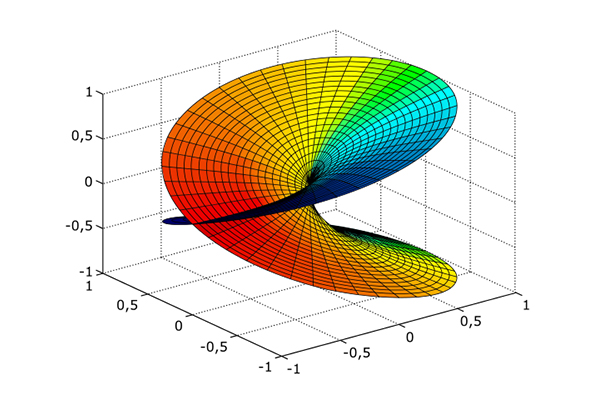
\includegraphics[width=0.7\linewidth]{immagini/riemann.jpg}
		\caption{Superficie di Riemann}
		\label{fig:riemann}
	\end{figure}
	\noindent Le due copie di $\C$ vanno incollate lungo quello che prima era il branch cut. In questo modo attraversando le linee di congiungimento si passa da un ramo all'altro. \newline
	In generale ci sono tante copie di $D \in \mathbb{C}$ quante sono le branch-cut (eventualmente anche infinite [es:~$\log(z)]$)
	\chapter{Integrazione sul piano complesso}	
	Le proprietà di olomorfia di $f(z)$ su $\mathbb{C}$ possono essere determinate dalle condizioni di Riemann. \newline
	Le proprietà di differenziabilità sono connesse con le proprietà di integrabiltà di $f(z) \mbox{ su } \mathbb{C}$ 
	\section{Curve}
	\begin{Def}[\textbf{Curva}] \hfil\\
		Una curva è una mappa continua 
			\begin{gather*}
				\gamma:[a,b] \in \mathbb{R} \rightarrow \mathbb{C} \\
				t \mapsto \gamma(t)= x(t) +iy(t)
			\end{gather*}	
		$z_a = \gamma(a) \mbox{ e } z_b=\gamma(b)$ sono gli estremi della curva 
	\end{Def}
	\begin{Def}[\textbf{Orientazione curva}] \hfil
		\begin{itemize}
			\item Una curva si dice che ha ORIENTAZIONE POSITIVA se il verso di percorrenza è antiorario
			\item Una curva si dice che ha ORIENTAZIONE NEGATIVA se il verso di percorrenza è orario
		\end{itemize}
	\end{Def}
	\begin{Def}[\textbf{Curva opposta}]\hfil\\
		La curva con orientazione opposta è data da una mappa 
		\[t \mapsto \gamma(a+b-t)=-\gamma\]
	\end{Def}
	\begin{Def}[\textbf{Curva semplice}]\hfil\\
		Una curva semplice è una curva che non si interseca $\Rightarrow$ mapping iniettivo
		\[\gamma(t_1)\neq\gamma(t_2) \quad \forall t_1\neq t_2\]
	\end{Def}
	\begin{Def}[\textbf{Curva chiusa}]\hfil\\
		Una curva chiusa è una curva tale che $\gamma(a)=\gamma(b)$ 
	\end{Def}
		\begin{Def}{\textbf{Curva di Jordan}}\hfil\\
		Una curva di Jordan è una curva semplice e chiusa (nessun altro punto oltre a $z_a=z_b$ coincide)
	\end{Def}
	\begin{Def}{\textbf{Curva regolare a tratti}}\hfill\\
		Data una curva $\gamma(t)=x(t)+iy(t)$, se $x(t) \mbox{ e } y(t)$ sono continue per $t\in[a,b]$ e se esiste una partizione di $[a,b]$ dove $x'(t) \mbox{ e } y'(t)$ sono continue e non simultaneamente nulle $\Rightarrow$ $\gamma(t)$ è regolare a tratti.
	\end{Def} 
	\begin{Def}{\textbf{Curve omotope}}\hfil\\
		Due curve su $D \in \mathbb{C}$ con gli stessi estremi $[a,b]$ sono omotope se: esiste una mappa continua che manda l'una nell'altra
		\begin{gather*}
			\gamma:[a,b]\times[0,1] \mapsto D \in \mathbb{C} \mbox{ t.c. se } t=[a,b] \mbox{ e } u=[0,1]: \\
			\forall t \in [a,b] \mbox{ } \forall u \in [0,1] \Rightarrow \gamma(t,0) = 	\gamma_1(t) \mbox{ e } \gamma(t,1)= \gamma_2(t)
		\end{gather*}
		Quindi $\gamma(a,u)=\gamma_1(a)=\gamma_2(a) \mbox{ e } \gamma(b,u)=\gamma_1(b)=\gamma_2(b)$ \newline
		Per ogni valore di u ho una curva in D; variando u passo da $\gamma_1$ a $\gamma_2$ 
	\end{Def} 
		\begin{teo}[\textbf{Jordan}]\hfil\\
			Ogni curva di Jordan divide il piano complesso in 2 regioni. \newline
			Se l'orientazione della curva è positiva a destra ho la regione esterna, mentre a destra ho la regione interna; se l'orientazione è negativa ho l'opposto. 
		\end{teo}
		\begin{Def}{\textbf{Dominio semplicemente connesso}}\hfil\\
			Date due curve $\gamma_1$ e $\gamma_2$ che sono omotope 
			\begin{equation*}
					\forall u \in [0,1] \Rightarrow \gamma(a,u)=\gamma(b,u) \mbox{ e } \gamma(t,0)=\gamma_1(t) 	\mbox{ } \gamma(t,1)=\gamma_2(t)
			\end{equation*}
			Allora il dominio D è semplicemente connesso se ogni curva chiusa è omotopa ad un punto (cioè può essere deformata in punto). \newline
			Ciò è possibile solo se non ci sono buchi.
		\end{Def}
	\section{Integrale di linea}
	\begin{Def}[\textbf{Integrale di linea}]\hfil\\
		Data una curva regolare a tratti $\gamma: t\mapsto\gamma(t)=x(t)+iy(t) \text{ con } t \in [a,b]\subseteq\mathbb{C}$ \newline
		Dato un dominio $D\subseteq\mathbb{C}$ e una funzione $f(z) \mbox{ con } z=\gamma(t)$ che sia continua $\forall z=\gamma(t)\in D \mbox{ e } \forall t \in [a,b]$ $\Rightarrow$ si definisce INTEGRALE DI LINEA di f lungo $\gamma$
		\begin{equation*}
		\int_\gamma f(z)\,dz = \int_{a}^{b} f(\gamma(t))\gamma'(t)\,dt \quad \mbox{ con }\gamma'(t) = \frac{d\gamma(t)}{dt} = x'(t)+iy'(t)
		\end{equation*}
		Si ha dunque 
		\begin{equation*}
			\int_\gamma f(z)\,dz = \int_{a}^{b} \bigl[u(x(t),y(t)) + iy(x(t),y(t))\bigr]\bigl(x'(t)+iy'(t)\bigr)\,dt \quad \text{con } f(z)= u(x,y)+iv(x,y)
		\end{equation*}
		\begin{equation*}
		\int_\gamma f(z)\,dz = \int_{a}^{b} (ux'-vy')\,dt + i\int_{a}^{b} (uy'+vx')\,dt
		\end{equation*}
	\end{Def}
	\begin{oss}
		Questo ci dice l'integrale è lineare e i cammini possono essere sommati
		\begin{gather*}
			\int_\gamma af(z)+bf(z)\,dz = a\int_\gamma f(z)\,dz + b\int_\gamma f(z)\,dz \quad \forall a,b \in \mathbb{C} \\
			\int_{\gamma_1} f(z)\,dz + \int_{\gamma_2} f(z)\,dz = \int_{\gamma_1+\gamma_2} f(z)\,dz \quad \mbox{se } \gamma_1(b)=\gamma_2(a)
		\end{gather*}
		Questa proprietà mi permette di scrivere $	\int_\gamma f(z)\,dz= -\int_{-\gamma} f(z)\,dz$
	\end{oss}
	\begin{oss}
		L'integrale è indipendente dalla parametrizzazione scelta per la curva $\gamma$
	\end{oss}
	\begin{Def}[\textbf{Lunghezza curva}]
		\begin{equation*}
			L=\int_{a}^{b} \abs{\gamma'(t)}\,dt = \int_{a}^{b} \sqrt{(x'(t))^2+(y'(t))^2}\,dt
		\end{equation*}
	\end{Def} 
	\begin{teo}[\textbf{Disuguaglianza di Darboux}]\hfil\\
		Data una curva regolare a tratti $\gamma(t)$ di lunghezza L e una funzione $f(z)$ continua e limitata su $\gamma$
		\begin{equation}
			\abs{f(z)}\le M \quad \forall z \in \gamma \Rightarrow \abs*{\int_\gamma f(z)\,dz}\le LM
		\end{equation}
	\end{teo}

\section{Valore principale integrale}
	Generalizzo il concetto di integrale improprio \newline
	se $f(z)$ è continua su una curva $\gamma(t)$ con $t\in [a,b]$ ad eccezione di un punto $\xi \in \gamma(t)$ \newline
	Posso considerare una circonferenza di raggio $\epsilon$ intorno a $\xi$ \newline
	Definisco 
	\begin{equation*}
		I_a = \int_{a}^{\xi'} f(\gamma(t))\gamma'(t)\,dt \text{ e } I_b = \int_{\xi''}^{b} f(\gamma(t))\gamma'(t)\,dt \quad \forall \epsilon>0	
	\end{equation*}
	Se esistono $I_a, I_b \mbox{ per } \epsilon\to 0 \Rightarrow I_a + I_b$ è integrale improprio di $f(z)$ lungo $\gamma$ \newline
	Se $I_a \mbox{ o } I_b \to\pm\infty \mbox{ quando } \epsilon \to 0 \mbox{ ma } \displaystyle \lim_{\epsilon\to 0} I_a + I_b = a (finito) \in \mathbb{C}
	\Rightarrow$ si definisce il valore principale 
	\begin{equation*}
		P.V. \int_\gamma f(z)\,dz = \lim_{\epsilon \to 0} \Bigl(\int_{a}^{\xi'(t)} f(z)\,dz + \int_{\xi''(t)}^{b} f(z)\,dz\Bigr)
	\end{equation*}

	\begin{nb}
		Se le singolarità sono più di una si può scrivere
		\begin{equation*}
			P.V. \int_\gamma f(z)\,dz =\lim_{\epsilon \to 0} \Bigl(\sum_{j=0}^{n} \int_{\xi''_j}^{\xi''_{j+1}} f(z)\,dz\Bigr) \quad \text{con } \xi''_0=a \quad \xi'_{n+1}=b
		\end{equation*} 
	\end{nb}
 
\chapter{Forme differenziali}
	\begin{Def}[\textbf{Forma differenziale}]\hfil\\
		$\omega = P(x,y)dx + Q(x,y)dy \quad$ con P,Q funzioni $C^1 \mbox{ su } D \subseteq \mathbb{R}^2$
	\end{Def}

	\begin{Def}[\textbf{Integrale di una forma differenziale}]\hfil\\
		L'integrale di una forma differenziale su una curva $\gamma(t)$ regolare a tratti è:
		\begin{equation*}
			\int_\gamma \omega = \int_{a}^{b} \bigl[P(x(t),y(t))x'(t)+Q(x(t),y(t))y'(t)\bigr]\,dt \Rightarrow \int_\gamma \omega = \int_\gamma f(z)
		\end{equation*} 
	\end{Def}
	
	\begin{teo}[\textbf{Green}]\hfil\\
		Data una forma differenziale definita su S racchiuso da una curva di Jordan $\gamma$ con orientazione positiva 
		\begin{equation}
			\int_\gamma P(x,y)dx + Q(x,y)dy\,dt = \iint_S \bigl[\delta_x Q(x,y)- \delta_y P(x,y)\bigr]\,dx\,dy
		\end{equation}
	\end{teo}

	\begin{teo}[\textbf{Cauchy}]\hfil\\
		Sia $f(z)$ olomorfa su D semplicemente connesso e $\gamma$ una curva chiusa in D 
		\begin{equation*}
			\int_\gamma f(z)\,dz = 0
		\end{equation*}
	\end{teo}

	\begin{oss}
		Esiste un'estensione dovuta a Goursat che non richiede che $f(z)$ sia derivabile su un dominio semplicemente connesso, ma basta chiedere che $f(z)$ sia omotopa ad un punto.
	\end{oss}

	\begin{coro}
		L'integrale di una funzione $f(z)$ olomorfa su D semplicemente connesso non dipende dal cammino $\gamma$
	\end{coro}

	\begin{oss}
		In generale se D non è semplicemente connesso il teorema fallisce.
	\end{oss}
	\begin{teo}\hfil\\
		Sia $f(z)$ olomorfa su un dominio D. Per un punto arbitrario $z_0 \in D $ possiamo sempre definire la primitiva 
		\begin{equation*}
			F(z)=\int_{z_0}^{z} f(z')dz
		\end{equation*}
		$F(z)$ è anch'essa olomorfa e si ha che $F'(z)= f(z)$
	\end{teo}

	\begin{coro}\hfil
		\begin{enumerate}
			\item Due diverse primitive di $f(z)$ possono differire solo per una costante.
			\item $\int_{A}^{B} f(z)\,dz = F(B)-F(A)$
		\end{enumerate}
	\end{coro}

\section{Relazione tra forme differenziali e campi vettoriali}
	Usando le condizioni di Cauchy-Riemann la forma differenziale su può scrivere come:
	\[\omega = f(z)dz = (u+iv)dx + (-v+iu)dy\]

	\begin{Def}[\textbf{Forma differenziale chiusa}]\hfil\\
		$\omega = P(x,y)dx + Q(x,y)dy$ \quad si dice chiusa se $\delta_y P = \delta_x Q$
	\end{Def}

	\begin{Def}[\textbf{Forma differenziale esatta}]\hfil\\
		$\omega = dg = \delta_x g(x,y)dx + \delta_y g(x,y)dy$
	\end{Def}

	\begin{oss}
		Ogni forma differenziale esatta è anche chiusa: $\delta_x\delta_y g(x,y) = \delta_y\delta_x g(x,y)$
	\end{oss}
\section{Formula integrale di Cauchy}

	\begin{teo}\hfil\\
		Data $f(z)$ olomorfa su D semplicemente connesso e data $\gamma$ di Jordan con orientazione positiva 
		\[\Rightarrow \forall z_0 \mbox{ interno a } \gamma \text{ si ha: } \quad 
		f(z_0) = \int_\gamma \frac {f(z_0)}{z-z_0} \,dz\]
	\end{teo}

	\begin{oss}
		Questo permette di costruire il valore di $f(z)$ all'interno di $\gamma$ partendo dai valori di $\gamma$ che sono il bordo della regione $\Rightarrow$ OLOGRAFIA
	\end{oss}

	\begin{coro}
		Se $f(z)$ è olomorfa in $z_0$ $\Rightarrow$ è differenziabile infinite volte e ha derivate che si possono scrivere come: 
		\[f^{(n)}(z_0)= \frac{n!}{2\pi i} \int_\gamma \frac{f(z)}{(z-z_0)^{n+1}} \, dz\]
		La formula integrale di Cauchy è un caso particolare per curve semplici e chiuse. Se la curva non è semplice si può avvolgere più volte attorno a $z_0$
	\end{coro}

	\begin{Def}[\textbf{Numero avvolgimenti}]
		\[n(\gamma,z_0) = \frac{1}{2 \pi i} \int_\gamma \frac{1}{z-z_0}\,dz \quad
		\Rightarrow \quad n(\gamma,z_0)f(z_0) = \frac{1}{2 \pi i} \int_\gamma \frac{f(z)}{z-z_0}\,dz\]
	\end{Def}

	\begin{teo}\hfil\\
		Data $\gamma(t)$ con $t \in [a,b]$ curva chiusa e dato $z_0 \notin \gamma$ si ha che $n(\gamma,z_0) \in \mathbb{Z}$
	\end{teo}

	\begin{Def}[\textbf{Funzione analitica}]\hfil\\
		Se $F(z)$ è olomorfa su un cerchio $D_R$ di raggio R attorno a $z_0 \in \mathbb{C}$ è anche analitica, cioè si può espandere in serie di potenze ed è derivabile infinite volte 
		\[f(z) =\sum_{n=0}^{\infty} a_n (z-z_0)^n \quad \mbox{con } a_n = \Bigl[\frac{d^n f(z)}{dz^n}\Bigr]_{z=z_0}\frac{1}{n!} = \frac{1}{2\pi i} \int_{D_R} \frac{f(z)}{(z-z_0)^{n+1}}\,dz\]
		R è il raggio di convergenza della serie.
	\end{Def}

	\noindent Il teorema di Cauchy mostra che $f(z)$ olomorfa su D semplicemente connesso implica che $\int_\gamma f(z)\,dz = 0$ con $\gamma$ curva di Jordan. \newline
	Il teorema di Morera afferma che le sole funzioni con queste proprietà sono le funzioni olomorfe.
	
	\begin{teo}{\textbf{Morera}}\hfil\\
		Data $f(z)$ su D semplicemente connesso tale che $\int_\gamma f(z)\,dz = 0$ con $\gamma$ curva semplice e chiusa \newline $\Rightarrow f(z)$ è olomorfa
	\end{teo}

	\paragraph{Ulteriori proprietà delle funzioni olomorfe}
	
	\begin{teo}[\textbf{valor medio}]\hfil\\
		Sia $f(z)$ olomorfa su $D \subset \mathbb{C}$ semplicemente connesso è possibile calcolare il vaolore di $f(a)$ tramite un integrale su di una qualsiasi circonferenza centrata in a e contenuta in D
		\[f(a)= \frac{1}{2\pi} \int_{0}^{2\pi} f(a+re^{i\theta})\,d\theta\]
		Cioè calcolando il valor medio della funzione sulla circonferenza
	\end{teo}

	\begin{Def}[\textbf{Bordo}]\hfil\\
		Dato uno spazio topologico S ed un punto $z_0 \in S$. Si dice che $z_0$ è un punto di bordo di S se ogni intorno di $z_0$ contiene sia punti di S che punti del suo complementare. \newline
		L'insieme dei punti di bordo si chiama BORDO e si indica con $\delta S$
	\end{Def}

	\begin{teo}[\textbf{massimo modulo}]\hfill\\
		Sia $f(z)$ olomorfa e non costante su un dominio D limitato tale che $f(z)$ sia continua sul bord $\delta D$ \newline $\Rightarrow$ $\abs{f(z)}$ raggiunge il massimo per un punto $z_0 \in \delta D$. Se $f(z) \neq 0 \Rightarrow$ anche il minimo è sul bordo.
	\end{teo}

	\begin{nb}
		Bisogna richiedere che f(z) sia diverso da zero perchè se $f(z_0) = 0 \mbox{ per } z_0 \in D \Rightarrow$ il minimo sarebbe $z_0$
	\end{nb}

	\begin{teo}[\textbf{Liouville}]\hfil\\
		Una funzione $f(z)$ olomorfa e limitata su $\mathbb{C}$ è una costante
	\end{teo}

	\begin{teo}[\textbf{fondamentale dell'algebra}]\hfil\\
		Un polinomio complesso di grado n ha esattamente n zeri sul piano complesso
	\end{teo}

	\begin{teo}[\textbf{unicità}]\hfil\\
		Sia $f(z)$ olomorfa su $D \subseteq \mathbb{C}$ non necessariamente semplicemente connesso tale che $f(z_n)=0 \forall$ elemento della successione ${z_n} \in D \mbox{ con } z_n \neq z_0$ punto di convergenza della serie allora:
		\[f(z)=0 \quad \forall z \in D\]
		Quindi tutti gli zeri di una funzione olomorfa sono punti isolati
	\end{teo}

	\begin{oss}
		è cruciale che $z_0 \in D$
	\end{oss}

	\begin{coro}
		Se $f(z)$ olomorfa è nulla su un aperto contenuto in D $\Rightarrow$ è nulla su tutto D
	\end{coro} 

	\section{Serie di Laurent}
	Olomorfie e analiticità sono proprietà che sui complessi sono connesse; una funzione olomofa è scrivibile in serie di Taylor
	\[ \label{eq:taylor}
	f(z) =\displaystyle \sum_{n=0}^{\infty} a_n(z-z_0)^n
	\]
	$\forall z_0 \in D \mbox{ in } f(z_0)$ sia olomorfa e $\forall$ disco $|z-z_0|<R$ interamente contenuto in D
	\[a_n = \Bigl[\frac{1}{n!} f^{(n)}(z)\Bigr]_{z=z_0} = \int_\gamma \frac{1}{2\pi i} \frac{f(z)}{(z-z_0)^n} \,dz\] 
	con $\gamma$ curva chiusa e semplice che contiene $z_0$
	
	\begin{oss}
		$f(z)$ è analitica perchè può essere differenziata infinite volte
	\end{oss}

	\begin{nb}
		Questa cosa non succede invece sui reali
	\end{nb}

	\noindent Per domini non semplicemente connessi è possibile dare una rappresentazione in serie di una funzione olomorfa su un anello \newline
	Applicazione $\rightarrow$ quando ci sono singolarità isolate \newline
	La serie che si ottiene è uan serie bilatera e si chiama SERIE DI LAURENT
	
	\begin{teo}\hfil\\
		Data $f(z)$ olomorfa su un anello $k = \{{z \in \mathbb{C} \mbox{ }| \mbox{ } r< |z-z_0|<R}\} \mbox{ con } z_0$ centro e r<R raggi \newline
		Si può allora scrivere la serie di Laurent 
		\begin{equation}
			f(z) = \sum_{n=-\infty}^{+\infty} d_n (z-z_0)^n = \underbrace{\sum_{n=0}^{+\infty} d_n(z-z_0)^n}_{parte regolare}  + \underbrace{\sum_{n=1}^{+\infty} \frac{d_n}{(z-z_0)^n}}_{parte principale}
		\end{equation}
		$d_n = \frac{1}{2\pi i } \int_\gamma \frac{f(z)}{(z-z_0)^{n+1}}\,dz \qquad$ con $\gamma$ curva semplice e chiusa su k con orientazione positiva
	\end{teo}

	\begin{nb}
		$ d_n \neq \bigl[\frac{1}{n!} f^{(n)}(z)\bigr]_{z=z_0}$ perchè la serie non contiene più solo potenze positive. \newline
		Quindi i coefficienti non si possono più scrivere in termini di semplici derivate perche $z_0$ uò essere una singolarità
	\end{nb}

	\begin{oss}
		I valori massimi e minimi dei raggi r e R sono:
		\[R =\Bigl(\lim_{n \to \infty} \sup_{k\ge n} |d_k|^{\frac{1}{k}}\Bigr)^{-1} \quad \mbox{con } n \ge 0\] 
		Cioè la parte regolare è una serie di potenze con n positiva che converge su $\abs{z-z_0}<R$
		\[ r =\Bigl(\lim_{n \to \infty} \sup_{k\ge n} |d_k|^{\frac{1}{k}}\Bigr) \quad \mbox{con } n > 1\]
		Cioè la parte principale è una serie di potenze $\omega = \frac{1}{z-z_0}$ che converge sul disco $\abs{\omega}<\frac{1}{r}$ \newline
		\noindent L'intersezione delle due regioni dà $r< \abs{z-z_0}<R$; quindi la serie converge uniformemente sull'anello k e su ogni suo sottoanello
	\end{oss}

	\noindent Data una singolarità isolata $z_0$ di $f(z)$ esiste un anello $k = \{z \in \mathbb{C} \mbox{ | } 0< |z-z_0|<\delta\}$ su $f(z)$  è olomorfa  e quindi esiste la sua espansione in serie di Laurent \newline
	\noindent La forma della serie dà informazioni su natura della singolarità
	
	\begin{enumerate}
		\item se $z_0$ è rimovibile $\Rightarrow$ la parte principale è assente e la serie coincide con la serie di Taylor (sostituisco la funzione con la sua serie di Taylor e rimuovo la singolarità)
		\item se $z_0$ è un polo di ordine k $\Rightarrow$ la parte principale contiene solo i primi k termini 
		\[f(z) = \sum_{n = -k}^{\infty} d_n (z-z_0)^n\]
		$d_{-k} = 0 \mbox{ } \forall k>n \mbox{ e } d_{-n} \neq 0$ solo polo più alto
		\item se $z_0$ è una singolarità essenziale la serie di Laurent contiene infiniti termini nella parte principale con potenze negative
	\end{enumerate}
	
\section{Prolungamento analitico}
	Data $f(z)$ olomorfa su $D \subset \mathbb{C}$ è possibile estendere estenderla su $D' \mbox{ con } D \subset D'$. Questo significa che data $f(z)$ con $z \in D$ si può trovare una funzione olomorfa $g(z)$ con $z \in D'$ tale che $f(z) = g(z) \mbox{ in } D \cap D'$ 
	$\Rightarrow$ si può definire $\tilde{f}(z)$ tale che:
	\[\tilde{f}(z) =
	\begin{cases}
			f(z) & \forall z \in D\\
			g(z) & \forall z \in D'
	\end{cases}\]
	Si ha che  $\tilde{f}(z)$ è olomorfa su $D \cup D'$ e si riduce a $f(z)$ su 
	
	\begin{Def}[\textbf{Prolungamento analitico}]\hfil\\
		La funzione  $\tilde{f}(z)$ è detto PROLUNGAMENTO ANALITICO di f
	\end{Def}

	\begin{teo}\hfil\\
		Se  $\tilde{f}(z)$ esiste $\Rightarrow$ è unico
	\end{teo}

\subsection{Massimo dominio di olomorfia}
	Ci sono diversi modi per calcolare la continuazione analitica; ognuno di questi metodi è valido in un sottodominio del massimo possibile
	
	\begin{enumerate}
		\item ESTENSIONE PER SERIE DI POTENZE \newline
		Si usa il metodo di Weierstrass (estensione per cerchi)
		
		\noindent Supponiamo di avere $f$ olomorfa su $D_0$ disco centrato nell'origine 0 con una singolarità $z_0$ sul bordo $\delta D_0$ \newline
		Preso $z_1 \in D_0$ posso espandere in serie di Taylor attorno a $z_1$ con raggio di convergenza  \newline $R_1 = \abs{z_1 - z_0}$ \newline
		Chiamo la serie di Taylor $f_1(z)$ e per costruzione $f(z) = f_1(z) \qquad \forall D_0 \cap D_1$ \newline
		Se $D_1$ non è interamente contenuto in $D_0$ $\Rightarrow f_1(z)$ è prolungamento analitico di $f$
		\begin{equation*}
			f_1(z) = \sum_{n=0}^{\infty} {\frac{1}{n!} f^n(z)\Big|_{z=z_1}(z-z_1)^n}
		\end{equation*}  
		Posso ripetere l'operazione e definire
		\begin{equation*}
			f_2(z) = \sum_{n=0}^{\infty} {\frac{1}{n!} f^n(z)\Big|_{z=z_2}(z-z_2)^n}
		\end{equation*}  
		Posso continuare fino al massimo dominio di olomorfia
		
		\item RAPPRESENTAZIONE INTEGRALE \newline
		Scrivo le funzioni in termini di un integrale
		\begin{equation}
			\Gamma(z) = \int_{0}^{\infty} e^{-t} t^{z-1}\,dt \quad \mbox{ FUNZIONE GAMMA DI EULERO}
		\end{equation}
		La funzione $\Gamma(z)$ generalizza il fattoriale ai numeri complessi
		
		\item ESPRESSIONE ANALITICA
	\end{enumerate}

\section{Residui}
	Vogliamo generalizzare il teorema di Cauchy al caso in cui $\int_\gamma f(z)\,dz$ sia su una curva chiusa che racchiude una singolarità di $f(z)$
	\begin{Def}[\textbf{Residuo}]\hfil\\
		Il residui di $f(z)$ nel punto $z_0$ di singolarità isolata con $f(z)$ altrimenti olomorfa su $D - \{z_0\}$ è definito come:
		\begin{equation*}
			Res[f,z_0] = d_{-1} 
		\end{equation*}
		con $d_{-1}$ coefficiente del termine $\frac{1}{z-z_0}$ nell'espansione di Laurent di $f(z)$ attorno a $z_0$. Cioè:
		\begin{equation*}
			Res[f,z_0] = \frac{1}{2 \pi i} \int_\gamma f(z)\,dz
		\end{equation*}
		con $\gamma$ semplice e chiusa con orientazione positiva che racchiude $z_0$
	\end{Def}

	\begin{oss}
		Il residuo può essere 0, per esempio $d_{-1} = 0 \mbox{ ma } d_{-n} \neq 0 \quad n>1$
	\end{oss}

	\begin{oss}
		Se $z_0$ è un polo di ordine k allora si ha:
		\begin{equation*}
			Res[f,z_0] = \frac{1}{(k-1)!} \lim_{z \to z_0} \frac{d^{k-1}}{dz^{z-k}} [(z-z_0)^kf(z)]
		\end{equation*}
	\end{oss}

	\begin{oss}
		Quando $f(z) = \frac{h(z)}{g(z)} \quad$ con $h(z)$ olomorfa e $g(z)$ ha unico zero semplice in $z_0$ dove $h(z_0) \neq 0$ allora:
		\begin{equation*}
			Res[f,z_0] = \frac{h(z_0)}{g'(z_0)}
		\end{equation*}
	\end{oss}

\subsection{Residuo all'infinito}
	Abbiamo visto che $f(z)$ può avere una singolarità isolata in $ z=\infty$. Si definisce allora il residuo all'infinito prendendo una circonferenza $\gamma = \{z \in \mathbb{C} \quad \vert \quad \abs{z}=R \} \quad$ con R grande a sufficienza a contenere tutte le singolarità al finito
	\begin{equation*}
		Res[f,\infty] = \frac{1}{2 \pi i } \int_{-\gamma} f(z)\,dz  
	\end{equation*} 
	$z=\infty$ può essere mappato in $w=0$ tramite $ w = \frac{1}{z}$
	\begin{equation*}
		Res[f,\infty] = \frac{1}{2 \pi i } \int_{-\gamma} f(z)\,dz = -\int_{\gamma'} \frac{1}{w^2}f\Bigl(\frac{1}{w}\Bigr)\,dw 
	\end{equation*} 
	con $\gamma'$ una circonferenza centrata in $w=0$ con raggio $\frac{1}{R}$ con orientazione positivaù
	\begin{equation*}
		Res[f,\infty] = 	Res\Bigl[g(w) = -\frac{1}{w^2} f\Bigl(\frac{1}{w}\Bigr),0\Bigr]
	\end{equation*}

	\begin{oss}
		Il $Res[f,\infty] \neq 0$ anche se $f(z=\infty)$ non è singolare
	\end{oss}

	\begin{teo}[\textbf{residui}]\hfil\\
		Data $f(z)$ olomorfa su D eccetto un numero finito di singolarità isolate $z_1,\dots,z_n$ e data una curva chiusa e semplice $\gamma \subset D$ con orientazione positiva si ha: 
		\begin{equation}
			\int_\gamma f(z)\,dz = 2 \pi i \sum_{k=1}^{n}Res[f,z_k] 
		\end{equation}
	\end{teo}

	\begin{coro}
		Quando $\gamma$ non è semplice o non è orientata positivamente si ha in generale:
		\begin{equation*}
			\int_\gamma f(z)\,dz = 2 \pi i \sum_{k=1}^{n} n(\gamma, z_k)Res[f,z_k] \qquad \textrm{n: indice con segno}
		\end{equation*}
	\end{coro}

	\begin{oss}
		Il teorema dei residui è utile perchè permette di calcolare l'integrale di funzioni olomorfe lungo una curva chiusa sapendo solo i valori della funzione alle singolarità racchiuse dalla curva
	\end{oss}

	\begin{coro}
		La somma di tutti i residui incluso il punto all'infinito è zero
	\end{coro}

	\begin{nb}
		Il teorema dei residui si può applicare solo quando $\gamma$ racchiude un numero finito di singolarità. Se fossero infinite ci potrebbe essere un punto di accumulazione per le singolarità che quindi non sarebbero più isolate. Per questo motivo il teorema dei residui non si può applicare direttamente alle funzioni multi-valued. Si può però applicare ad ogni brach basta stare attenti che $\gamma$ non attraversi il branch-cut
	\end{nb}

\section{Valore principale di Cauchy}

	Se abbiamo singolarità sul cammino di integrazione $\int_{-\infty}^{\infty} \frac{f(x)}{x-x_0}\,dx$ con $x_0 \in \R \text{ e } f(x)$ regolare in $x_0$ tale che $\displaystyle \lim_{x \to \pm\infty} f(x) \to 0$ sufficientemente rapido. \newline
	Si può definire il valore principale di Cauchy 
	\[P.V. \int_{-\infty}^{\infty} \frac{f(x)}{x-x_0}\,dx = \lim_{\epsilon \to 0^+} \Bigl[\int_{-\infty}^{x_0-\epsilon}\frac{f(x)}{x-x_0} + \int_{x_0+\epsilon}^{\infty} \frac{f(x)}{x-x_0}\Bigr]\]
	I due integrali sono separatamente divergenti, ma nella somma la divergenza in $\epsilon$ si cancella. \newline
	Calcolo integrale usando $\Gamma_R$
	\begin{figure}[H]
		\centering
		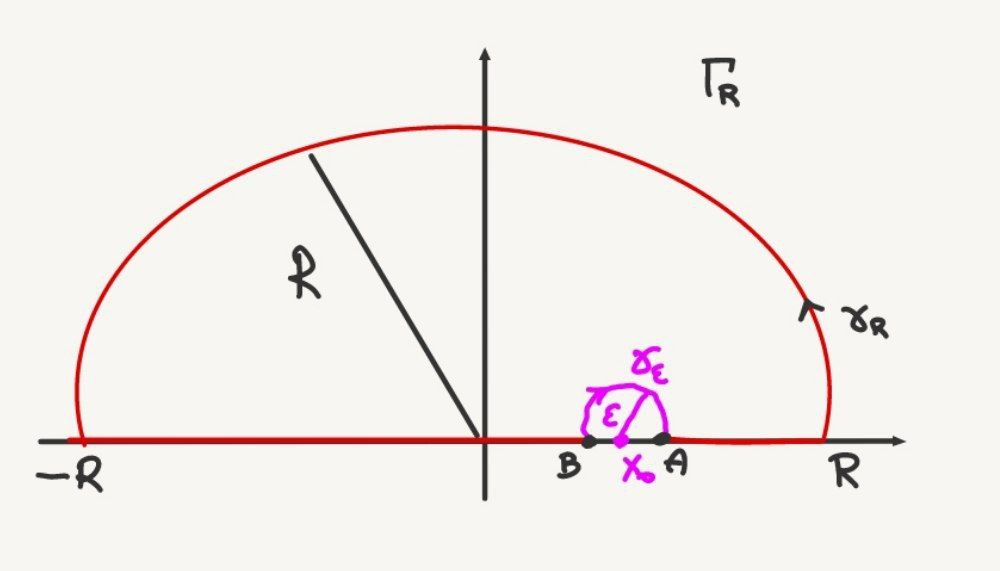
\includegraphics[width=0.5\linewidth]{immagini/fig1}
		\label{fig:fig1}
	\end{figure}

	\[I(R) = \int_{\Gamma_R} \frac{f(z)}{z-x_0}\,dz = 2\pi i \sum_k Res\Bigl[\frac{f(z)}{z-x_0},z_k\Bigr]\]
	Allora
	\begin{equation}
		P.V. \int_{-\infty}^{\infty} \frac{f(x)}{x-x_0}\,dx = \pi i f(x_0) + 2\pi i \sum_k Res\Bigl[\frac{f(z)}{z-x_0},z_k\Bigr]
	\end{equation}

\chapter{Proprietà mapping}

	Una funzione $f(z)$ può essere vista come una mappa da $\C \rightarrow \C$ \newline
	Dato un aperto $\Omega \subseteq D$ dominio di olomorfia, studio comportamento locale di $f$ per capire cosa succede a $f(\Omega) = \{f(z) \quad \vert \quad z \in \Omega\}$: \newline
	f è olomorfa $\Rightarrow$ f è analitica $\Rightarrow$ f è sviluppabile in serie di Taylor attorno a $z_0 \in \Omega$ \newline
	Il comportamento locale di f ha determinato dai primi termini della \hyperref[eq:taylor]{serie di taylor} \newline
	m è il primo indice tale che $a_m \neq 0$ $\Rightarrow$ il comportamento locale è determinato da 
	\[f(z)-f(z_0) \simeq a_m(z-z_0)^m\]
	Ci sono due casi:
	
	\begin{enumerate}
		\item $m=1$ \quad cioè \quad $a_1=f'(z_0)\neq0$
		
		\begin{teo}\hfil\\
			Esiste un aperto $U$ in un intorno di $z_0$ tale che:
			\begin{itemize}
				\item $f \text{ mappa } U$ in un intorno di $f(U)$ in maniera biunivoca
				\item $f(U)$ è un aperto $\Rightarrow$ f è una mappa aperta
				\item $f$ ha una funzione inversa $f^{-1}$ olomorfa e manda $f(U) \rightarrow U$
				\item $f$ è una mappa CONFORME, cioè converva gli ancoli tra le linee
			\end{itemize}
		\end{teo}
	
		\begin{Def}
			Dire che gli angoli si preservano significa che se le rette L e L' hanno angolo $\theta$ fra loro su U $\Rightarrow$ $f(L)$ e $f(L')$ hanno tangenti che si intersecano con angolo $\theta$ su $f(U)$ 
		\end{Def}
	
		$f$ manda rette in curve, ma le tangenti preservano gli angoli
		
		\begin{oss}
			Dato che $f^{-1}$ è olomorfa allora si può espandere in serie di Taylor attorno a $w_0=f(z_0)$
			\[f^{-1}(w) = \sum_{k=0}^{\infty} b_k (w-w_0)^k\]
			con i $b_k$ dati dalla formula di Lagrange
			\[b_0 = z_0 \qquad b_n = \frac{1}{n!} \frac{d^{n-1}}{dz^{n-1}} {\Bigl(\frac{z-z_0}{f(z)-f(z_0)}\Bigr)}^n \Bigr|_{z=z_0} \, n\geq 1\]
		\end{oss}
	
		\item $m>1$ si può dimostrare che esiste un aperto $U$ tale che 
		\begin{itemize}
			\item $f$ è una mappa m a 1 
			\item $f(U)$ è un aperto
			\item $f$ ingrandisce gli angoli di un fattore m
		\end{itemize}
	
	\end{enumerate}

	\begin{teo}[\textbf{Open Mapping}]\hfil\\
		Ogni funzione $f$ olomorfa non costante mappa aperti in aperti
	\end{teo}

	\begin{nb}
		Questo non vale se la funzione è costante perchè $f$ mappa $\C$ in un punto
	\end{nb}

	\begin{teo}\hfil\\
		Se $f$ è olomorfa e biunivoca si ha: 
		\[f'(z_0) \neq 0\ \; \forall z  \qquad \exists \, f^{-1} \text{ olomorfa }\]
		Si dice che $f$ è una MAPPA CONFORME
	\end{teo}

\section{Trasformazioni lineari fratte}
	Trasformazioni lineari conformi del tipo:
	\[F(z) = \frac{az + b}{cz + d} \qquad a,b,c,d \in \C\]
	con $ad-cb \neq 0$ sono mappe conformi $\forall z_0$ tali che $z_0 \neq -\frac{b}{c}$ \newline
	Inoltre
	\[F'(z) = \frac{ad-bc}{{cz+d}^2} \neq 0 \]
	Casi particolari:
	\begin{enumerate}
		\item Traslazioni: \qquad $w = z + \alpha$
		\item Dilatazioni: \qquad $w = \beta z$
		\item Inversioni:  \qquad $w = \frac{1}{z}$
	\end{enumerate}
	Qualsiasi $f$ lineare fratta può essere scitta come combinazione di queste 3 trasformazioni
	\begin{oss}
		Spesso conviene esprimere $F(z)$ sulla sfera di Riemann $\hat{\C} = \C \cup \{\infty\}$
		\[F\left(-\frac{d}{c}\right) = \infty \quad F(\infty) = \frac{a}{c} \qquad \text{quando } c=0 \to \infty\]
		Allora le trasformazioni lineari fratte sono le uniche mappe biunivoche e olomorfe di $\hat{\C} \rightarrow \hat{\C}$ \newline
		Sono AUTOMORFISMI  di $\hat{\C}$ \newline
		Mappano rette e cerchi in se stessi (in realtà su $\hat{\C}$ le rette sono cerchi che passano da $\infty$) \newline
		Inoltre dati 3 punti $z_1,z_2,z_3$ e dati $w_1,w_2,w_3$ esiste una sola trasformazione F che abbia 
		\[w_i = F(z_i) \; i=1,2,3\]	
	\end{oss}
	\begin{nb}
		\[B(z,z_1,z_2,z_3) = \frac{(z-z_1)(z_2-z_3)}{(z-z_3)(z_2-z_1)}\]
		è invariante sotto trasformazioni lineari fratte
		\[B(F(z),F(z_1),F(z_2),F(z_3)) = B (z,z_1,z_2,z_3)\]
	\end{nb}
	\begin{oss}
		L'insieme delle trasformazioni $F$ forma un gruppo. Associamo a $F$ la matrice 
		\[
		\hat{F} = 
		\left(\begin{matrix}
			a & b \\ c & d
		\end{matrix}\right)
		\qquad F = \frac{az + b}{cz+d}
		\]
		Inversa e composizione di $F$ seguono dalle regole delle matrici \newline
		Dato che si può riscalare $\hat{F} \rightarrow \lambda \hat{F}$ con $\lambda \in \C$ senza cambiare trasformazione allora si può normalizzare $\hat{F}$ in modo che $ ad-cb = 1$ \newline
		Quindi il gruppo delle trasformazioni $F$ è $SL(2, \C)$ gruppo di matrici $2 \times 2$ complesse e determinante unitario \newline
		Dato che $\det \hat{F} = 1$ non fissa il segno di $a,b,c,d$ ho che il gruppo è:
		\[\frac{Sl(2,\C)}{\mathbb{Z}_2} \qquad \mathbb{Z}_2 = \{\mathbb{I}, - \mathbb{I}\}\] 
	\end{oss}
	\begin{teo}[\textbf{Riemann mapping}]\hfill\\
		Ogni aperto semplicemente connesso $\omega \subset \C$ può essere mappato conformemente (cioè usando $f$ bi-olomorfa) sul cerchio unitario aperto
	\end{teo}
	\begin{coro}
		Tutte le regioni aperte di $\C$ semplicemente connesse sono uniformemente equivalenti 
	\end{coro}

\part{Spazi funzionali}

Vogliamo estendere la definizione di spazi euclidei $\R^3$ in maniera astratto in mdo da poterli usare anche per spazi$\infty-$dimensionali

\begin{Def}
	Uno \textbf{SPAZIO VETTORIALE V} su uno campo F è un insieme con 3 operazioni, chiuso rispetto:
	\begin{enumerate}
		\item somma per elementi dello spazio (vettori)
		\[\forall \, \vec{v},\vec{w} \in V \Rightarrow \vec{v}+\vec{w} \in V\]
		\item moltiplicazione per un elemento di F (scalari)
		\[\forall \lambda \in F \; \forall \, \vec{v}\in V \Rightarrow \lambda\vec{v} \in V\]
	\end{enumerate}
\end{Def}

\noindent La somma di vettori è associativa, commutativa, con elemento neutro $\vec{0}$ e inverso -$\vec{v}$; inoltre è distributiva sul prodotto con $\lambda \in F$ 
\[\lambda (\vec{v}+\vec{w}) = \lambda\vec{v}+\lambda\vec{w}\]
e ha elemento neutro prodotto $1\in F$

\begin{Def}
	$W \subset V$ è un \textbf{SOTTOSPAZIO} di V se è chiuso rispetto alla somma e moltiplicazione per uno scalare
	\begin{gather*}
		\forall\, \vec{v}, \vec{w} \in W \Rightarrow \vec{v}+\vec{w}\in W \subset v \\
		\forall \, \vec{v} \in W \; \forall \lambda \in F \Rightarrow \lambda \, \vec{v} \in W \subset V 
	\end{gather*}
\end{Def}

\begin{Def}
	n vettori $\vec{u}_k \; k = 1, \dots , n$ sono \textbf{lineramente indipendenti} se 
	\[\sum_{k=1}^n a_k \vec{u}_k = 0 \Rightarrow \forall k = 1,\dots,n 	\; a_k=0\]
\end{Def}

\begin{Def}
	Invece sono \textbf{lineramente dipendenti} se 
	\[\sum_{k=1}^n a_k\vec{u}_k = 0 \qquad \text{con qualche } a_k \ne 0\]
\end{Def}

\begin{Def}
	Un insieme di vettori linearmente indipendenti è detto \textbf{massimale} se l'insieme dei vettori linearmente indipendeti + uno qualsiasi altro vettore è linearmente dipendente \newline
	\{$u_k$\} è chiamata \textbf{base} di V
\end{Def}

\begin{oss}
	Data una base posso scrivere un qualsiasi vettore $\vec{v}\in V$ in coordinate o componenti
	\[\vec{v} = \sum_{k=1}^n v_k\vec{u}_k \qquad v_k \in F\]
\end{oss}

\begin{oss}
	n può essere finito o infinito; se è finito tutte le basi hanno lo stesso numero di vettori e si chiama \textbf{dimensione} dello spazio \newline
	Gli spazi di funzioni sono un esempio di spazio $\infty-$dimensionali
\end{oss}

\noindent Sugli spazi vettoriali astratti è possibile aggiungere strutture che permettorno di specificare il concetto di lunghezza o distanza, il concetto di limite e di continuità in maniera astratta

\begin{Def}
	Una \textbf{metrica o distanza} è una mappa 
	\[d(,): \, M \to \R\]
	con le seguenti proprietà valide $\forall a,b \in M$
	\begin{gather*}
		d(a,b) = d(b,a) \\
		d(a,b) = 0 \iff a=b \\
		\forall c \in M \quad d(a,b)+d(b,c) \ge d(a,c)
	\end{gather*}
\end{Def}

\begin{Def}
	Uno spazio vettoriale i cui è possibile definire una matrica è uno \textbf{spazio metrico}
\end{Def}

\begin{Def}
	Una \textbf{topologia} su un insieme X è una collezione $\tau$ di sottoinsiemi di X che contiene l'insieme vuoto, X stesso e che deve essere chiusa rispetto ad un numero finito di iterazioni e ad un numero arbitrario di interazioni, cioè
	\begin{itemize}
		\item $\emptyset \in \tau$
 		\item $X in \tau$
		\item $\forall \, V_i \in Z \quad V_1 \cap V_2 \cap \dots \cap V_n \in \tau $
		\item $\cup_\alpha \quad V_\alpha \in \tau$ \; con $\alpha$ finito o infinito
	\end{itemize} 
	Gli elementi di $\tau$ sono gli insiemi aperti 
\end{Def}

\begin{oss}
	La topologia non è unica
\end{oss}

\begin{Def}
	Una \textbf{sfera aperta} di raggio r centrata in $a \in M$ è
	\[B(a,r) = \{b \in M \; | \; d(a,b)<r\}\]
\end{Def}

\begin{Def}
	Ogni sottoinsieme di $X\subset M$ è aperto se 
	\[\forall \, a_o \in X \quad \exists \, B(a_o,r) \subset X\]
\end{Def}

\begin{oss}
	Ogni spazio metrico è uno spazio topologico, basta definire la topologia degli aperti tramite sfere aperte
\end{oss}

\begin{Def}
	Un insieme è \textbf{chiuso} se il suo complementare è aperto
\end{Def}

\begin{oss}
	L'esistenza di una topologia metrica permette di definire la nozione di limite di una successione \;
	Diciamo che \{$a_n$\} converge ad $a\in M$ se 
	\[\forall \varepsilon>0 \quad \exists \, n_o \text{ tale che } d(a_n, a)<\varepsilon \quad \forall \, n>n_o\]
	oppure usando la definizione di limite di $\R$
	\[\lim_{n\to \infty} d(a_n,a) =0\]
\end{oss}

\begin{oss}
	La convergenza di una serie si prova con la convergenza delle somme parziali
\end{oss}

\begin{oss}
	Un insieme chiuso contiene tutti i suoi punti di accumulazione ed il più piccolo insieme chiuso che contiene X è detto \textbf{chiusura} di X ($\bar{X}$)
\end{oss}

\begin{Def}
	Un insieme Z si dice \textbf{denso} in Y se la sua chiusura corrisponde a $Y = \bar{Z}$
\end{Def}

\begin{Def}
	Un insieme K in uno spazio metrico X è \textbf{compatto} $\iff$ ogni succesione \{$X_k$\} interamente contenuta in K ha una sottosuccesione convergente ad un elemento di K
\end{Def}

\begin{Def}
	Una mappa
	\[f: \; X\to Y\]
	tra due spazi topologici è \textbf{continua} se la controimmagine di ogni aperto in Y contenente f($X_0$) è un aperto in X contenente $X_0$ \newline
	Per spazi metri è possibile formulare ciò con sfere aperte
	\[\forall\varepsilon> 0 \quad \forall \delta> 0 \text{ tale che } d(f(x),f(x_0))<\varepsilon \qquad \text{ se } d(x,x_0)<\delta\]
\end{Def}

\begin{Def}
	Una \textbf{successione di Cauchy} è una succesione \{$x_n$\} tale che 
	\[\forall \varepsilon>0 \quad \exists \; N_\varepsilon >0 \text{ tale che } \forall \; n,m \ge N_\varepsilon \qquad d(x_n,x_m)< \varepsilon\]
\end{Def}

\begin{teo}
	In uno spazio metrico ogni successione convergente è una successione di Cauchy 
\end{teo}

\begin{Def}
	Uno spazio metrico si dice \textbf{completo} se tutte le successioni di Cauchy sono convergenti 
\end{Def}

\chapter{Spazi normati}

\begin{Def}
	La \textbf{norma} di un vettore $\in V$ spazio vettoriale è una mappa
	\[||\,||: \; V \to \R^+\]
	che soddisfa $\forall \; \vec{v},\vec{w}\in V \quad \forall\lambda \in \C,\R$
	\begin{enumerate}
		\item $||\vec{v}||\ge 0 \qquad ||{\vec{v}}||=0 \iff \; \vec{v} = \vec{0}$ \qquad condizione di positività
	  	\item $||\lambda\vec{v}|| = \abs{\lambda}||\vec{v}||$
    \item $||\vec{v}+\vec{w}|| \le ||\vec{v}|| + ||\vec{w}||$ \qquad disuguaglianza triangolare
	\end{enumerate}
\end{Def}

\begin{Def}
	Uno spazio vettoriale dotato di norma si dice \textbf{spazio normato}
\end{Def}

\begin{coro}
	Gli spazi normati sono sempre degli spazi metrci dato che si può sempre definire
	\[d(\vec{v},\vec{w})= ||\vec{v}-\vec{w}||\]
\end{coro}

\begin{coro}
	Per la convergenza in uno spazio normato si può usare 
	\[\lim_{n\to\infty} ||\vec{v}_n - \vec{v}|| =0\]
\end{coro}

\begin{Def}
	Un \textbf{isomorfismo} tra spazi normati è una mappa biunivoca
	\[f: \; (X, ||\,||_x) \to (Y, ||\, ||_y)\]
	che preserva la struttura lineare e la norma, cioè
	\begin{itemize}
		\item $f(\lambda\vec{v}+\mu\vec{w}) = \lambda f(\vec{v})+ \mu f(\vec{w})$ 
  \item $||f(\vec{v})||_y = ||\vec{v}||_x \qquad \forall \;\vec{v},\vec{w} \in X \quad \lambda,\mu \in F$
	\end{itemize}
\end{Def}

\begin{oss}
	Tramite la norma superiore 
	\[||f||_{sup} = \sup_{x\in K} \abs{f(x)}\]
	possiamo definire il concetto di convergenza uniforme
\end{oss}

\begin{Def}
	$\{f_n\} \to f$ converge uniformemente su K se 
	\[\lim_{n\to\infty} \underbrace{\sup_{x\in K} \abs{f_n(x)-f(x)}}_{||f_n-f||_{sup}} =0\]
\end{Def}

\begin{oss}
	La convergenza uniforme inplica la convergenza puntuale
\end{oss}

\begin{Def}
	Norma $L_1$
	\[||f||_1 = \int_0^1 \abs{f(x)}\, dx\]
\end{Def}

\begin{oss}
	Si può dimostrare che la convergenza in norma sup implica convergenza in norma $L_1$
\end{oss}

\begin{Def}
	Uno \textbf{spazio di Banach} è uno spazio vettoriale normato e completo
\end{Def}

\begin{Def}
	Il \textbf{prodotto scalare (o interno)} su uno spazio vettoriale complesso è una mappa 
	\begin{align*}
		(\vec{a},\vec{b}): \; V\times V &\to \C \\
		\vec{v},\vec{w} &\mapsto (\vec{v},\vec{w})
	\end{align*}
	che soddisfa le seguenti proprietà:
	\begin{enumerate}
		\item Linearità
		\[(\vec{u}, \lambda\vec{v}+\mu\vec{w}) = \lambda(\vec{u}, \vec{v}) + \mu(\vec{v},\vec{w}) \qquad \forall\lambda,\mu \in \C\]
		\item Hermiticità \label{2}
		\[(\vec{v}, \vec{w}) = \overline{(\vec{w},\vec{v})} \quad \text{ simmetria su $\R$}\]
		\item Positività
		\[(\vec{v},\vec{v})\ge 0 \qquad (\vec{v},\vec{v})=0 \iff \vec{v} = \vec{0}\]
	\end{enumerate}
\end{Def}

\begin{oss}
	La prop \hyperref[2]{2} implica anti-linearità nel primo argomento
	\[(\lambda\vec{u}+\mu\vec{v}, \vec{w}) = \bar{\lambda}(\vec{u},\vec{w})+\bar{\mu}(\vec{v},\vec{w})\]
\end{oss}

\begin{Def}
	Uno spazio vettoriale dotato di prodotto scalare è detto \textbf{pre-Hilbert}
\end{Def}

\begin{oss}
	Pre-Hilbert è anche uno spazio normato; si può sempre definire
	\[||\vec{v}|| = \sqrt[]{(\vec{v}, \vec{v})}\]
\end{oss}

\begin{oss}
	Il prodotto scalare soddisfa la disuguaglianza di Schwarz
	\[{\abs{(\vec{v},\vec{w})}}^2 \le (\vec{v},\vec{v})(\vec{w},\vec{w})\]
\end{oss}

\begin{Def}
	Uno \textbf{spazio di Hilbert finito dimensionale} è uno spazio vettoriale dotato di prodotto scalare e completo 
\end{Def}

\begin{Def}
	Due vettori sono \textbf{ortogonali} se il loro prodotto scalare è nullo
	\[(\vec{v},\vec{w})=0\]
\end{Def}

\begin{oss}
	I vettori ortogonali sono linearmente indipendenti 
\end{oss}

\begin{oss}
	Gli elementi di una base (set massimale di vettori linearmenti indipendenti) sono \textbf{ortomormali}
	\[(\vec{e}_i,\vec{e}_j) = \delta_{ij} \quad \forall \; i,j = 1,\dots,n\]
	\begin{enumerate}
		\item $\vec{v} = \displaystyle \sum_{k=1}^n v_k \vec{e}_k \qquad v_k = (\vec{e}_k,\vec{v})$
  \item $(\vec{v},\vec{w})= \displaystyle \sum_{k=1}^n \bar{v}_k\vec{w}_k \qquad \bar{v}_k = (\vec{v}, \vec{e}_k) \quad \vec{w}_k = (\vec{e}_k,\vec{w})$
  \item ${||\vec{v}||}^2 = \displaystyle \sum_{k=1}^n {\abs{v_k}}^2$ identità di Parseval
	\end{enumerate}
\end{oss}

\begin{oss}
	In ogni spazio di Hilbert finito dimensionale è sempre possibile costruire una base ortonormale a partire da qualsiasi base 
\end{oss}

\chapter{Spazi di Hilbert infinito dimensionali}
Ci concentriamo sugli spazi separabili, cioè che hanno un sottoinsieme denso che è contabile \newline
Diciamoc che il set $\{\vec{l}_k\}$ con $k\in \mathbb{N}$ in uno spazio di Hilbert infinito dimensionale è un sistema ortonormale Se
\[(\vec{e}_i,\vec{e}_j) = \delta_{ij} \quad \forall \, i,j \in \mathbb{N} \]
Se inoltre $\forall \vec{v}$ si può scrivere
\[\vec{v} = \sum_[i=1]^\infty v_i\vec{e}_i \qquad v_i = (\vec{e}_i,\vec{v})\in \C\]
allora il sistema $\{\vec{e}_k\}$ è un \textbf{sistema ortonormale completo} [S.O.N.C] o base di Hilbert

\begin{oss}
	Abbiamo generalizzato la nozione di base usando $\infty$ elementi; ciò è possibile perchè abbiamo la nozione di limite
	\[\vec{v} = \lim_{n\to\infty} \sum_{i=1}^n v_i\vec{e}_i \qquad \vec{v} = \lim_{n\to\infty} \left|\left| \sum_{i=1}^n v_i\vec{e}_i - \vec{v}\right| \right| =0\] 
\end{oss}

\begin{Def} \label{Fourier}
	L'espansione 
	\[\vec{v} = \sum_{i=1}^\infty (\vec{e}_i,\vec{v})\vec{e}_i\]
	è chiamata \textbf{serie di Fourier} e i coefficienti $v_i$ sono detti coefficienti di Fourier
\end{Def}

\begin{teo}
	La serie $\displaystyle \sum_{i=1}^n \alpha_i\vec{e}_i$ converge $\iff \displaystyle \sum_{i=1}^\infty {\abs{\alpha_i}}^2$ converge 
\end{teo}

\begin{oss}
	Come nel caso finito dimensionale valgono
	\begin{itemize}
		\item $(\vec{v},\vec{e}_i) = 0 \quad \forall i \Rightarrow \vec{v}=0$
  \item $||\vec{v}|| = \displaystyle \sum_{k=1}^\infty {\abs{v_k}}^2 \quad \forall\vec{v}$
  \item $\forall \; \vec{v},\vec{w} \in V \Rightarrow (\vec{v},\vec{w}) = \displaystyle \sum_{k=1}^\infty \bar{v}_kw_k$
	\end{itemize}
\end{oss}

\begin{Def}
	Lo spazio $l^2(\C)$
	\[\sum_{n=1}^\infty {\abs{z_n}}^2 < \infty\]
	è uno spazio di Hilbert con il prodotto scalare \newline
	In generale gli spazi $l^p(\R)$ o $l^p(\C)$ con $1 \le p <\infty$
	\[\sum_{n=0}^\infty {\abs{x_n}}^p < \infty\]
	sono solamente dotati di norma, quindi sono spazi di Banach 
\end{Def}

\begin{oss}
	Si può dimostrare utilizzando la disuguaglianza di Minkowski per le serie 
	\[{\left(\sum_{n=0}^\infty {\abs{x_n+y_N}}^p\right)}^{\frac{1}{p}} \le {\left(\sum_{n=0}^\infty {\abs{x_n}}^p\right)}^{\frac{1}{p}} + {\left(\sum_{n=0}^\infty {\abs{y_n}}^p\right)}^{\frac{1}{p}}\]
\end{oss}

\begin{Def}
	Gli spazi $l^\infty(\R/\C)$ sono anch'essi spazi di Banach formati da successioni limitate e dotati di norma superiore
	\[\sup_{0\le n \le \infty} \abs{x_n} < \infty\]
\end{Def}

\noindent Il tipico esempio di prodotto scalare su spazi di Hilbert infinito dimensionale è quello di funzioni sull'intervallo $[a,b]$
\[(f,g) = \int_a^b \bar{f}(x)g(x) \, dx\]
La somma $L^1$ rientra in questa categoria

\section{Integrali}
\subsection*{Integrale di Riemann}
\[I = \sum_{i=1}^n (x_{i+1}-x_i)f(\bar{x}_i)\]
Quando esiste finito il limite per $n \to \infty \; x_{i+1}-x_i \to \infty$ si dice INTEGRALE DI RIEMANN  e la funzione si dice integrabile secondo Riemann 

\subsection*{Integrale Lebesgue}
\[I = \sum_{i=1}^n f_i\mu (f^{-1}([f_{i+1}-f_i]))\]
con $f_i$ una partizione del range di f e con $\mu(x)$ misura di X \newline
La controimmagine di un intervallo non è necessariamente un intervallo 

\chapter{Spazio \texorpdfstring{$L^1_w (\Omega)$}{U}}
\begin{Def}
	Lo spazio $L^1_w(\Omega)$ è uno spazio di funzioni definite su un insieme $\Omega\subset \R/\C$, Lebesgue-integrabili con norma
	\[||f||_1 = \int_\Omega \abs{f(x)}\underbrace{w(x)}_{misura} \, dx <\infty\]
\end{Def}

\noindent Questi spazi $L^1_w(\Omega)$ sono spazi di Banach 

\begin{oss}
	Lo spazio delle funzioni continue su un intervallo $C([a,b])$ con norma 
	\[L^1 = \int_a^b f(x) \, dx \]
	non è uno spazio di Banach, perchè non è completo 
\end{oss}

\begin{oss}
	Se vogliamo che lo spazio $L^1_w(\Omega)$ sia uno spazio di Banach dobbiamo provare linearità, positività e disuguaglianza triangolare nella norma $L^1_w$ \newline
	La linearità e la disuguaglianza trinagolare seguono facilmente dalle proprietà degli integrali, la positività vera per integrale di Riemann, ma non è più vera in generale per integrale di Lebesgue; dobbiamo allora definire $f(x)=0$ quasi ovunque
\end{oss}

\begin{teo}[Riesz-Fischer] \label{teo:riesz}
	$L^1_w$ è completo e quindi di Banach 	
\end{teo}

\begin{nb}
	Per dimostrare che questo spazio è completo, bisogna usare ben due teoremi dell'integrale di Lebesgue $\Rightarrow$ questo vale solo per funzioni Lebesgue-integrabili 
\end{nb}

\section{Spazi \texorpdfstring{$L^p_w(\Omega)$}{U}}
Spazio delle funzioni a valori complessi du regione $\Omega \subset \R^n/\C^n$ tale che 
\[\int_\Omega {\abs{f(x)}}^p w(x)\, dx < \infty \qquad p \ge 1 \in \R \]

\begin{oss}
	Le funzioni uguali quasi ovunque sono considerate identiche
\end{oss}

\begin{oss}
	Gli spazi $L^p_w(\Omega)$ sono spazi di Banach con norma $L^p_w$
	\[||f||_p = {\left(\int_\Omega {\abs{f(x)}}^p w(x) \, dx \right)}^{\frac{1}{p}}\]
	La completezza di questi spazi si può dimostrare generalizzando il \hyperref[teo:riesz]{teorema di Riesz-Fischer}
\end{oss}

\begin{oss}
	Ci sono due ulteriori disuguaglianze notevoli; se assumiamo che p e q siano coniugati, cioè $\frac{1}{p} + \frac{1}{q} = 1$ allora valgono
	\begin{enumerate}
		\item Disuguaglianza di Holder
		\[||fg||_p \le ||f||_p ||g||_p\]
		\item Disuguaglianza di Minkowski
		\[||f+g||_p \le ||f||_p + ||g||_p\]
	\end{enumerate}
\end{oss}

\begin{oss}
	Tra tutti i p possibili, il caso p=2 è particolare; $L^2_w(\Omega)$ non è solo uno spazio di Banach, ma anche uno spazio di Hilbert. E\' infatti l'unico su cui si può definire il prodotto scalare 
	\[(f,g) = \int_\Omega \bar{f}(x)g(x)w(x) \, dx \]
	che induce norma $L^2_w$
	\[||f||_2 = {((f,f))}^{\frac{1}{2}} = {\left(\int_\Omega {\abs{f(x)}}^2 w(x) \, dx\right)}^{\frac{1}{2}}\]
	$L^2_w(\Omega)$ è lo spazio delle funzioni a quadrato integrabile e contiene sia funzioni continue $C(\Omega)$ sia funzioni con singolarità  
\end{oss}

\chapter{Basi di Hilbert ed espansione di Fourier}

Applicando la teoria generale degli spazi di Hilbert a $L^2_w(\Omega)$ si arriva alla conclusione che è possibile definire una base contabile di funzioni in $L^2_w(\Omega)$ \newline
Quindi una qualsiasi funzione $f\in L^2_w(\Omega)$ può essere espressa come combinazione degli infiniti elementi della base ortogonale

\section{Basi ortonormali}

Una funzione si dice normalizzata se la sua norma è 1; in particolare per $L^2_w(\Omega)$

\begin{equation*}
	\label{eq:1.1}
	{||f||}_2 = \int_\Omega \abs{f(x)}^2w(x) \, dx = 1
\end{equation*}

\begin{Def}
	\label{def:ortogonali}
	Due funzioni sono \textbf{ortogonali} se 
	\begin{equation*}
		(f,g) = \int_\Omega \overline{f(x)}g(x)w(x) \, dx = 0
	\end{equation*}
\end{Def}

\begin{Def}
	\label{def: base ortonormale}
	Una \textbf{base ortonormale} è un set di funzioni $\Psi_n(x)$ con $n = 0,1,\dots,N$ su $L^2_w(\Omega)$ che soddisfano
	\begin{equation*}
		(\Psi_n,\Psi_m) = \delta_{m,n} \qquad \forall \; m,n = 0,1,\dots,N 
	\end{equation*}
\end{Def}

\begin{oss}
	Se non ci sono altre funzioni ortogonali a tutti $\Psi_n$ allora il sistema è completo. Quindi \{$\Psi_n$\} è una base di Hilbert di $L^2_w(\Omega)$
\end{oss}

\noindent Per la teoria generale degli spazi di Hilbert si può perciò espandere qualsiasi funzione $f\in L^2_w(\Omega)$ sulla base 
\begin{equation*}
	\sum_{n=0}^\infty C_n \Psi_n \qquad \text{serie di Fourier}
\end{equation*}
I coefficienti di Fourier $C_n$ si calcolano
\begin{equation*}
	C_n = (\Psi_n,f) = \int_\Omega \overline{\Psi_n(x)}f(x)w(x) \, dx 
\end{equation*}

\begin{oss}
	La convergenza della serie di Fourier non implica che 
	\begin{equation*}
		\sum_{n=0}^\infty C_n\Psi_n
	\end{equation*}
	converga puntualmente (cioè $\forall \, x$) ad f, ma va intesa come convergenza in norma $L^2_w(\Omega)$, cioè
	\begin{equation*}
		\lim_{n\to\infty} \int_\Omega {\abs{f(x) - \sum_{n=0}^n C_n\Psi_n}}^2 w(x) \, dx =0
	\end{equation*}
\end{oss}

\begin{oss}
	La serie di Fourier di una qualsiasi funzione a quadrato integrabile definita su $[a,b]$ converge alla funzione stessa in norma $L_2$
	\begin{equation*}
		\lim_{n\to\infty} {||\sum{k=-n}^n c_k \Psi_k - f||}_2 =0
	\end{equation*}
\end{oss}

\begin{oss}
	Se $f(x)\in\R \Rightarrow c_k = \overline{c}_{-k}$
\end{oss}

\begin{oss}
	La serie di Fourier su $L^2_{[a,b]}$ può essere anche scritta in forma trigonometrica usando 
	\begin{equation*}
		e^{\pm 2\pi in \frac{x}{L}} = \cos{\left(\frac{2\pi nx}{L}\right)} \pm i\sin{\left(\frac{2\pi nx}{L}\right)}
	\end{equation*}
	per cui 
	\begin{equation*}
		f(x) = \frac{a_0}{2} + \sum_{n=1}^\infty a_n \cos{\left(\frac{2\pi nx}{L}\right)} + \sum_{n=1}^\infty \sin{\left(\frac{2\pi nx}{L}\right)}
	\end{equation*}
	In questa formulazione i coefficienti sono dati da 
	\begin{gather*}
		a_n = \frac{c_n + c_{-n}}{\sqrt[]{2}} \qquad b_n = \frac{i(c_n - c_{-n})}{\sqrt[]{2}} \\
		a_n = \frac{2}{L} \int_a^b f(x) \cos{\left(\frac{2\pi nx}{L}\right)} \, dx \qquad  b_n = \frac{2}{L} \int_a^b f(x) \sin{\left(\frac{2\pi nx}{L}\right)} \, dx 
	\end{gather*}
	Quindi la base della forma trigonometrica è data da 
	\begin{equation*}
		\left\{\frac{1}{\sqrt[]{L}}, \sqrt[]{\frac{2}{L}} \cos{\left(\frac{2\pi nx}{L}\right)}, \sqrt[]{\frac{2}{L}} \sin{\left(\frac{2\pi nx}{L}\right)}\right\} \qquad n>1
	\end{equation*}
	Le funzioni della base trigonometrica si chiamano \textbf{armoniche} e il numero $\frac{n}{L}$ si dice frequenza dell'armonica
\end{oss}

\begin{oss}
	Per definire i coefficienti della serie di Fourier 
	\begin{equation*}
		c_n = \frac{1}{\sqrt[]{L}} \int_a^b e^{-2\pi i \frac{nx}{L}} f(x) \, dx
	\end{equation*}
	basta che $f(x)\in L^1_{[a,b]}$ e non per forza in $L^2_{[a,b]}$
\end{oss}

\section{Convergenza puntuale}

Per semplicità assumiamo $[a,b] = [0,2\pi]$ \newline
Se prendo $f(x)\in L^1_{[0,2\pi]}$ allora 
\begin{equation*}
	c_n =(\Psi_n,f) = \frac{1}{\sqrt[]{2\pi}}\int_0^{2\pi} e^{-inx} f(x)
\end{equation*}
sono ben definiti e si può costruire la serie di Fourier
\begin{equation*}
	\frac{1}{\sqrt[]{2\pi}} \sum_{n=-\infty}^\infty c_n e^{inx}
\end{equation*}
Osservo che la serie di Fourier ha termini che sono periodici con periodo $2\pi$
\begin{equation*}
	e^{inx} = e^{i(nx+2\pi)}
\end{equation*}
Quindi posso estendere le funzioni f da $[0,2\pi]$ a tutto $\R$ usando le condizioni periodiche per l'estensione
\begin{equation*}
	f(x+2\pi) = f(x)
\end{equation*}
Allora posso studiare su tutto $\R$ la convergenza delle somme parziali
\begin{equation*}
	S_n(x) = \frac{1}{\sqrt[]{2\pi}} \sum_{k=-n}^n c_ke^{-ikx} = \sum_{k=-n}^n \frac{1}{2\pi} \left[\int_0^{2\pi} e^{-iky}f(y) \, dy\right] e^{-ikx} = \frac{1}{2\pi}\int_0^{2\pi} \sum_{k=-n}^n e^{ik(x-y)}f(y) \, dy 
\end{equation*}
ora sfrutto la periodicità di f per cambiare variabile $z = x-y$ dato che 
\begin{equation*}
	\int_{a+2\pi}^{b+2\pi} f(x)\, dx = \int_a^b f(x) \, dx 
\end{equation*}
Allora ottengo
\begin{equation*}
	S_n(x) = \frac{1}{2\pi} \int_0^{2\pi} \sum_{k=-n}^n e^{ikz}f(x+z) \, dz
\end{equation*}
introduco KERNEL DI DIRICHLET
\begin{equation*}
	D_n(z) = \sum_{k=-n}^n e^{ikz} = \frac{\sin{\left(\frac{2n+1}{2}z\right)}}{\sin{\left(\frac{z}{2}\right)}}
\end{equation*}
per riscrivere
\begin{equation*}
	S_n = \frac{1}{2\pi} \int_0^{2\pi} f(x+z)D_n(z) \, dz
\end{equation*}
dividendo integrale ottengo
\begin{equation*}
	S_n(x) = \frac{1}{\pi} \int_0^\pi \frac{f(x+z)-f(x-z)}{2}D_n(z)
\end{equation*}

\begin{teo}[Dirichlet]\hfill\\
	Data f con periodo $2\pi$  che sia $L^1_{[0,2\pi]}$ tale che 
	\begin{equation*}
		\lim{y\to x^{\pm}} f(y) = f(x^{\pm})	
	\end{equation*}
	e tale che esista integrale 
	\begin{equation*}
		\int_0^\delta \frac{f(x\pm y)-f(x^{\pm})}{y} \, dy
	\end{equation*}	
	per qualche valore di $\delta$, allora la serie di Fourier 
	\begin{equation*}
		\frac{1}{\sqrt[]{2\pi}} \sum_{n=-\infty}^\infty c_n e^{inx}
	\end{equation*}
	converge a 
	\begin{equation*}
		\begin{cases}
			f(x) \qquad &\text{se f è continua}\\
			\frac{1}{2}[f(x^+)+f(x^-)] \qquad & \text{se f è discontinua}
		\end{cases}
	\end{equation*}
\end{teo}

\begin{oss}
	Il teorema di Dirichlet si applica a tutte le funzioni $C^1$ a pezzi 
\end{oss}

\chapter{Polinomi ortonormali}

Si può applicare metodo ortogonalizzazione di Gram-Schmidt anche a basi $\infty-$dimensionale. \newline
Solitamente si parte da monomi con potenze diverse: $1,x,x^2,x^3,\dots$ eventualmente moltiplicati per funzioni a decrescenza rapida per renderle integrabili a $\pm\infty$ \newline
Queste sono soluzioni linearmente indipendenti e tramite Gram-Schimdt si può arriavre a sestema ortormale completo su $L^2_w [a,b]$ \newline
Ci sono vari esempi di polinomi ortogonali, la cui forma dipende principalmente dall'intervallo $[a,b]$ e dalla misura $w(x)$
\begin{enumerate}
	\item $[a,b]$ finito, $w(x)=1 \Rightarrow$ $[-1,1]$ polinomi di Legendre
 \item $[0,\infty], \, w(x)=e^{-x} \Rightarrow$ polinomi di Laguerre
 \item $[-\infty,\infty], \, w(x) = e^{-x^2} \Rightarrow$ polinomi di Hermite
\end{enumerate}

\section{Polinomi di Legendre}
Ci focalizziamo sull'intervallo $[-1,1]$ (viene dal fatto che sono associati a soluzioni a simmetria sferica e rappresentano la dipendenza da $-1<\cos{\theta}<1$) \newline
I polinomi di Legendre si indicano con $P_l(x)$ o $P_l(\cos{(\theta)})$ e si possono ricavare dalla formula di Rodrigues
\begin{equation*}
	P_l(x) = \frac{1}{2^ll!}\frac{d^l}{dx^l}{(x^-1)}^l \qquad l\in \mathbb{N}
\end{equation*}
Si possono anche ricavare anche dalla funzione generatrice
\begin{equation*}
	F(x,t) = \frac{1}{\sqrt[]{1-2xt+t^2}} = \sum_{l=0}^\infty P_l(x)t^l
\end{equation*}
I polinomi di Legendre sono normalizzati in modo che 
\begin{equation*}
	P_l(1)=1
\end{equation*}
Si ha che i primi polinomi sono
\begin{equation*}
	P_0(x)=1 \qquad P_1(x)=x \qquad P_2(x)= \frac{1}{2}(3x^2-1)
\end{equation*}
in generale si ha $P_l(x)$ è un polinomio di grado massimo l in x \newline
Vale la relazione di parità
\begin{equation*}
	P_l(-x) = -1^lP_l(x)
\end{equation*}
I polinomi di Legendre soddisfano le seguenti relazioni ricorsive
\begin{align*}
	P'_{l+1}(x) &= (l+1)P_l(x)+xP'_l(x)\\
	P'_{l-1}(x) &= -lP_l(x)+xP'_l(x)\\
	(l+1)P_{l+1}(x) &= (2l+1)xP_l(x)-lP_{l-1}(x)
\end{align*}
Questi polinomi soddisfano un'equazione differenziale particolare che si chiama equazione di Legendre
\begin{equation*}
	(1+x^2)P''_l(x) - 2xP'_l(x)+l(l+1)P_l(x) =0
\end{equation*}
Ma la loro vera utilità è la condizione di ortogonalità
\begin{equation*}
	(P_l,P_m) = \int_{-1}^1 P_l(x)P_m(x) \, dx = \frac{2}{2l+1}\delta_{lm}
\end{equation*}
quindi posso definire le funzioni ortonormali
\begin{equation*}
	u_l(x)=\sqrt[]{\frac{2l+1}{2}}P_l(x)
\end{equation*}
tali che $\{u_l\}$ forma un sistema ortonormale completo, cioè una base di Hilbert di $L^2[-1,1]$

\begin{teo}[Approssimazione di Weierstrass]\hfill\\
	Ogni funzione continua f(x) su [a,b] limitato è il limite uniforme di una successione di polinomi $\{Q_n(x)\}$
\end{teo}

\begin{oss}
	Dato che i polinomi di Legendre sono una base di Hilbert di $L^2[-1,1]$ si può espandere una qualsiasi funzione su [-1,1] in serie di Fourier usando come base $u(x) = \sqrt[]{\frac{2l+1}{2}}P_l(x)$
	\begin{equation*}
		f(x) = \sum_{l=0}^\infty a_l u_l(x) = \sum_{l=0}^\infty a_l\,  \sqrt[]{\frac{2l+1}{2}}P_l(x) \qquad a_l = (u_l,f) = \sqrt[]{\frac{2l+1}{2}}\int_{-1}^1 P_l(x)f(x)\, dx 
	\end{equation*}
	si chiama sviluppo di Legendre di una funzione 
\end{oss}

\section{Polinomi di Laguerre}

I polinomi di Laguerre sono un S.O.N.C  per $L^2[0,\infty]$ con misura $w(x)= e^{-x}$. Si costruiscono ortogonalizzando con Gram-Schmidt i monomi $1,x,x^2,\dots$ e si ottiene
\begin{equation*}
	L_n(x) = \frac{e^x}{n!}\frac{d^n}{dx^n}[e^{-x}x^n] \qquad n\in \mathbb{N}
\end{equation*}
si possono anche definire tramite funzione generatrice 
\begin{equation*}
	F(x,t) = \frac{e^{-\frac{xt}{1-t}}}{1-t} = \sum_{n=0}^\infty L_n(x)t^n
\end{equation*}
I primi polinomi sono
\begin{equation*}
	L_0(x)=1 \qquad L_1(x)=1-x \qquad L_2(x)=\frac{1}{2}(x^2-4x+2)
\end{equation*}
in generale $L_n(x)$ è un polinomio di grado massimo n in x \newline
Gli $L_n(x)$ soddisfano le seguenti relazioni di ricorrenza
\begin{align*}
	L_{n-1}(x)&=L'_{n-1}(x)-L'_n(n)\\
	xL'_n(x) &= nL_n(x)- nL_{n-1}(x)\\
	(n+1)L_{n+1}(x) &= (2n+1-x)L_n(x)-nL_{n-1}(x)
\end{align*}
soddisfano inoltre l'equazione differenziale di Laguerre 
\begin{equation*}
	xL''_n(x) + (1-x)L'_n(x) + nL_n(x) =0
\end{equation*}
I polinomi sono ortogonali con misura $w(x)=e^{-x}$
\begin{equation*}
	(L_n,L_m) = \int_0^\infty L_n(x)L_m(x)e^{-x} \, dx = \delta_{nm}
\end{equation*}
Quindi le funzioni $L_n(x)$ sono un S.O.N.C. di $L^2_w[0,\infty]$ con $w = e^{-x}$, oppure si possono usare le funzioni $L_n(x)e^{-\frac{x^2}{2}}$ per fare un S.O.N.C. $L^2[0,\infty]$ con $w=1$

\section{Polinomi di Hermite}

Sono un S.O.N.C. per $L^2_w[-\infty,\infty]$ con $w(x) = e^{-x^2}$. Sono definiti da 
\begin{equation*}
	H_n(x) = {(-1)}^ne^{x^2}\frac{d^n}{dx^n}e^{-x^2} \qquad n\in \mathbb{N}
\end{equation*}
oppure tramite la funzione generatrice 
\begin{equation*}
	F(x,t) = e^{2xt-t^2}=\sum_{n=0}^\infty \frac{H_n(x)}{n!}t^n
\end{equation*}
I primi polinomi sono
\begin{equation*}
	H_0(x)=1 \qquad H_1(x) = 2x \qquad H_2(x)= 4x^2
\end{equation*}
In generale $H_n(x)$ sono polinomi di grado massimo n in x \newline
La parità dipende da n
\begin{equation*}
	H_N(-x)= {(-1)}^nH_n(x) 
\end{equation*}
Soddisfano le relazioni di ricorrenza
\begin{align*}
	H'_n(x) &= 2nH_{n-1}(x)\\
	H{n+1}(x) &= 2xH_n(x)-2nH_{n-1}(x)
\end{align*}
e soddisfano l'equazione differenziale di Hermite
\begin{equation*}
	H''_n(x)-2xH'_n(x)+2nH_n(x)=0
\end{equation*}
Per $n\ne m$ ho
\begin{equation*}
	(H_n,H_m) = \int_{-\infty}^\infty H_n(x)H_m(x)e^{-x^2} \, dx = 2^nn!\sqrt[]{\pi} \delta_{n,m}
\end{equation*}
Se voglio avere una base ortonormale devo normalizzare gli $H_n(x)$ tramite
\begin{equation*}
	h_n(x) = \frac{H_n(x)}{\sqrt[]{2^nn!\;\sqrt[]{\pi}}}
\end{equation*}
che sono un S.O.N.C. per $L^2[-\infty,\infty]$ \newline
Allo stesso modo si possono definire 
\begin{equation*}
	w_n(x)= h_n(x)e^{-\frac{x^2}{2}}
\end{equation*}
che sono un S.O.N.C. su $L^2[-\infty,\infty]$ con $w(x)=1$

\chapter{Trasformata di Fourier}

Richiamo \hyperref[Fourier]{serie di Fourier}

\noindent Si può definire la traformata di Fourier  $\forall \, f(x)\in L^1(\R)$ e si indica con
\begin{equation*}
	F(f)(p) \qquad \hat{f}(p)
\end{equation*}
ed è definita da
\begin{equation*}
	\hat{f}(p) = \frac{1}{\sqrt[]{2\pi}} \int_{-\infty}^\infty f(x)e^{-ipx} \, dx 
\end{equation*}
$\frac{1}{\sqrt[]{2\pi}}$ è un fattore di normalizzazione abbastanza arbitrario, ma l'importante è che sia consistente con l'antitrasformata \newline
Questa espressione è ben definta perchè se $f(x)\in L^1(\R)$ allora $f(x)e^{-ipx}\in L^1(\R)$ se $p\in\R$

\begin{oss}
	Nel caso di più variabili
	\begin{equation*}
		f(\vec{x}) = f(x_1,\dots,x_n) \Rightarrow \hat{f}(\vec{p}) = \frac{1}{{(2\pi)}^{\frac{N}{2}}}\int f(\vec{x})e^{-i(\vec{p},\vec{x})} \, dx_1,\dots,dx_n
	\end{equation*}
\end{oss}

\noindent Lo spazio di p si chiama \textbf{spazio coniugato allo spazio delle x} o anche \textbf{spazio duale}; in fisica si chiama spazio degli impulsi duale allo spazio delle posizioni ( o spazio di Fourier)

\section{Gaussiana}

\begin{equation*}
	\hat{f}(p) = \frac{1}{\sqrt[]{2\pi}} \int_{-\infty}^\infty e^{-ipx}e^{-\frac{x^2}{2a^2}}\, dx = ae^{-\frac{p^2}{2{\left(\frac{1}{a}\right)}^2}}
\end{equation*}

\noindent Quindi la trasformata di Fourier di una gaussina di larghezza a è ancora una gaussiana, ma di larghezza $\frac{1}{a}$; più la gaussiana originale è piccata attorno al suo valor medio, più la sua trasformata si allarga

\section{Funzione caratteristica}

Trasformata di Fourier della funzione caratteristica dell'intervallo $(-a,a)$
\begin{equation*}
	\hat{\chi}_a(x) = \,  \sqrt[]{\frac{2}{\pi}} \frac{\sin{(pa)}}{p}
\end{equation*}
la larghezza è proporzionale a $\frac{1}{a}$; più f(x) è piccata attorno al suo valor medio, più la trasformata si allarga

\section{Lorenztiana}

\begin{equation*}
	\hat{f}(p) = \, \sqrt[]{\frac{\pi}{2}}\frac{1}{a} e^{-\abs{p}a}
\end{equation*}

\section{Proprietà trasformata di Fourier}

\begin{enumerate}
	\item Linearità
	\begin{equation*}
		F(\alpha f + \beta g) = \alpha F(f) + \beta F(g)
	\end{equation*}
	\item F(f) è limitata, continua e si annulla all'infinito
 \item Derivata: se $f^{(k)}\in L^1(\R)$ allora la trasformata di Fourier della derivata k-esima esiste e vale
\begin{equation*}
	F(f^{(k)})(p) = {(ip)}^k F(f)(p)
\end{equation*}
\item Moltiplicazione per x: se $\abs{x}^kf(x) \in L^1(\R)$ allora la trasformata di Fourier esiste e vale 
\begin{equation*}
	F(x^kf)(p) = \int_{-\infty}^\infty \frac{1}{\sqrt[]{2\pi}} x^k f(x)e^{-ipx} \, dx 
\end{equation*}
quindi c'è una corrispondenza tra lo spazio delle posizioni e lo spazio degli impulsi
\begin{center}
\begin{tabular}[H]{|c|c|}
	\hline
	Spazio x & Spazio p \\
	\hline
	$\frac{d}{dx}$ & ip \\
	x & $i\frac{\delta}{\delta p}$ \\
	\hline
\end{tabular}
\end{center}
\item Trasformata di Fourier come convoluzione: se $f,g \in L^1(\R)$ allora $f*g \in L^1(\R)$ e la trasformata di Fourier esiste e vale
\begin{equation*}
	F(f*g)(p) = \int_{-\infty}^\infty f(y)g(x-y) \, dy = \sqrt[]{2\pi} F(f)F(g)
\end{equation*}
\end{enumerate}

\section{Trasformata di Fourier inversa}

\begin{teo}
	Data $f(x)\in L^1(\R)$ tale che $\hat{f}(p) \in L^1(\R)$ allora si può costruire f(x) data $\hat{f}(p)$ con la formula di inversione
	\begin{equation*}
		f(x) 0 \frac{1}{\sqrt[]{2\pi}} \int_{-\infty}^\infty e^{ipx}\hat{f}(p) \, dp
	\end{equation*}
	questa è l'estesione al continio della di Fourier per $p\in\R$
\end{teo}

\begin{oss}
	\'E sufficiente che $\hat{f}(p)$ si possa antitrasformare quai ovunque per definire f(x) quasi ovunque, cioè nel senso della norma $L^1$
\end{oss}

\begin{oss}
	Dato che gli elementi di $L^1(\R)$ sono classi di equivalenza di funzioni uguali quasi ovunque non ha senso affermare che il teorema di inversione valga puntualmente. Tuttavia la formula di inversione è una funzione continua in x, quindi data $f\in L^1(\R)$ tale che $\hat{f}p \in L^1(\R)$ allora esiste una funzione continua nella stessa classe di equivalenza ; se scegliamo f continua allora il teorema di inversione diventa valido puntualmente. In generale però se $ f \in L^1(\R)$ si può avere che $\hat{f}(p) \not\in L^1(\R)$; bisogna quindi modificare teorema di inversione e vederlo come limite
	\begin{equation*}
		\lim_{R\to\infty} \frac{1}{\sqrt[]{2\pi}} \int_{-R}^R \hat{f}(p)e^{ipx} \, dp
	\end{equation*}
	Tale limite può esistere anche quando $\hat{f}$ non è integrabile su tutto $\R$; inoltre si può dimostare che tale se $f \in L^1(\R)$ ed è continua a pezzi, allora si può dimostare che tale definizione porta a 
	\begin{equation*}
		\lim_{R\to\infty} \frac{1}{\sqrt[]{2\pi}} \int_{-R}^R \hat{f}(p) e^{ipx} \, dp = \begin{cases}
			f(x) & \forall\, x \text{ dove f è continua} \\
			\frac{f(x^+)+f(x^-)}{2} & \text{ dove f è discontinua}
		\end{cases}
	\end{equation*}
	notare similitudine con serie di Fourier per funzioni a pezzi
\end{oss}

\section{Trasformata di Fourier in \texorpdfstring{$S(\R)$ ed in $L^2(\R)$}{U}}

Data $f(x) \in L^2(\R)$ non si ha necessariamente $f \in L^1(\R)$ quindi la trasformata può non esistere, ma data $f \in S(\R)$ la trasformata esiste sempre perchè 
\begin{equation*}
	S(\R) \subset L^1(\R) 
\end{equation*}


\part{Distribuzioni}

\noindent  Distribuzione: concetto che generalizza ed estende il concetto di funzione

\begin{Def}
	Una \textbf{distribuzione} è un funzionale lineare, cioè una mappa
	\begin{equation*}
		T: \; \phi(x) \to T(\phi) \in \phi
	\end{equation*}
	da uno spazio di funzioni di prova $\phi(x)\in F$ (spazio delle funzioni di prova) al campo dei numeri complessi
\end{Def}

\noindent Ad ogni funzione f(x) si può associare il funzionale $T_f$ tale che 
\begin{equation*}
	\forall \phi(x) \in F \qquad T_f (\phi) = \int_{-\infty}^\infty f(x)\phi(x)\, dx 
\end{equation*}

\begin{oss}
	In generale si può usare funzionale lineare generale e possiamo definire su quest'ultimo operazioni che non possono essere ben definite sulla funzione di partenza 	 
\end{oss}

\chapter{Lo spazio delle funzioni di prova}

Vogliamo test functions di una sola variabile (estensione a più dimensioni è banale) e vogliamo inoltre che $\phi(x)\in F$ sia il più regolare possibile, quindi
\begin{equation*}
	\phi \in C^\infty(\R)
\end{equation*}
inoltre per garantire che per esempio
\begin{equation*}
	\int_{-\infty}^\infty f(x)\phi(x)\, dx < \infty
\end{equation*}
chiediamo che le $\phi$ siano soppresse a $\pm \infty$; come viene implementata questa richiesta determina lo spazio F 

\begin{enumerate}
	\item Spazio $D(\R)$ delle funzioni $C^\infty(\R)$ a supporto compatto
	\begin{Def}
		Il \textbf{supporto} è la chiusura dei punti in cui la funzione non è nulla
		\begin{equation*}
			supp\{f\}= \overline{\{x \in \R \; |\; f(x) \ne 0 \}}
		\end{equation*}
	\end{Def}
	\item Spazio $S(\R)$ delle funzioni $C^\infty(\R)$ a decrescenza rapida
\end{enumerate}

\section{Spazio \texorpdfstring{$D(\R)$}{U}}

\begin{equation*}
	D(\R) = \{\phi(x) \; | \; \phi \in C^\infty(\R) \text{ con supporto compatto}\}
\end{equation*}
Compatto in $\R$ significa chiuso e limitato

\begin{oss}
	$D(\R)$ è uno spazio vettoriale, ma è anche uno spazio topologico; tuttavia la topologia non è indotta dalla metrica. A noi interessa solo capire come definire la nozione di convergenza nello spazio topologico di $D(\R)$
\end{oss}

\begin{Def} \label{def: sequenza}
	Una \textbf{sequenza} di test functions \{$\phi_n\} \in D(\R)$ converge a $\phi \in D(\R)$ se valgono
	\begin{itemize}
		\item esiste un intervallo limitato $\hat{I} \subset \R$ che contiene il supporto di tutte le $\phi_n$
  		\item esiste un numero reale $r$ tale che 
		\begin{equation*}
			\phi_n(x) = \phi(x) =0 \qquad \forall \, \abs{x}>r 
		\end{equation*}
		\item la sequenza delle derivate p-esime di $\phi_n(x)$ converge uniformemente alla derivata p-esima di $\phi(x)$
		\begin{equation*}
			\lim_{n\to\infty} \sup_{x\in\R} \left|\frac{d^p\phi_n(x)}{dx^p}- \frac{d^p\phi(x)}{dx^p}\right| =0 \qquad \forall \, p=1,2,3,\dots
		\end{equation*}
	\end{itemize} 
\end{Def}

\begin{nb}
	$p=0$ significa $\phi_n \to \phi $ uniformemente
\end{nb}

\begin{oss}
	Tutte le funzioni $\phi(x)$ in $D(\R)$ non sono analitiche
\end{oss}

\begin{oss}
	$D(\R)\subset L^2(\R)$ perchè le $\phi$ sono a quadrato sommabile; inoltre $D(\R)$ è denso in $L^2(\R)$
\end{oss}

\section{Spazio \texorpdfstring{$S(\R)$}{U}}

\begin{equation*}
	S(\R) = \left\{\phi(x) \;| \; \phi \in C^\infty(\R) \text{ e } \lim_{x\to \pm\infty} x^p \frac{d^p}{dx^p}f(x)=0 \quad  \forall \, p,q = 0,1,2,\dots \right\}
\end{equation*}

\begin{Def}
	Una sequenza $\{\phi_n\} \in S(\R)$ \textbf{converge} a $\phi \in S(\R)$ se una qualsiasi potenza di x moltiplicata per una qualsiasi derivata di $\phi_n$ converge uniformemente ala stessa combinazione di x e derivate di $\phi$, cioè
	\begin{equation*}
		\forall \, p,q \qquad \lim_{n\to\infty} \sup_{x\in\R} \left|x^p \frac{d^p}{dx^p}\phi_n(x - x^p\frac{d^p}{dx^p}\phi(x))\right| =0
	\end{equation*}
\end{Def}

\begin{oss}
	Ogni $\phi\in S(\R)$ è a quadrato sommabile, quindi 
	\begin{equation*}
		S(\R) \subset L^2(\R)
	\end{equation*}
	in effetti $S(\R)$ è denso in $L^2(\R)$, cioè ogni elemento di $L^2(\R)$ può essere visto come limite di una successione di elementi di $S(\R)$
\end{oss}

\begin{Def}
	Chiamiamo \textbf{distribuzione} un funzionale che associa un numero complesso ad una test function
	\begin{equation*}
		\phi(x) \to T(\phi) \in \C
	\end{equation*}
	che ha le seguenti proprietà
	\begin{enumerate}
		\item è lineare
		\begin{equation*}
			T(\lambda_1\phi_1 + \lambda_2\phi_2) = \lambda_1T(\phi_1)+ \lambda_2T(\phi_2) \qquad \forall\phi_1,\phi_2 \in D(\R)\text{ o } S(\R) \quad \forall \lambda_1,\lambda_2 \in \C 
		\end{equation*}
		\item è continua, nel senso che data una sequenza di test functions $\{\phi_n\}\in F$ che converge a $\phi\in F$ si ha
		\begin{equation*}
			\lim_{n\to\infty} T(\phi_n) = T(\phi)
		\end{equation*}
	\end{enumerate}
\end{Def}

\begin{Def}
	Se $\phi\in D(\R)$ allora $T(\phi)$ si chiama \textbf{distribuzione} e lo spazio vettoriale definito dai T è chiamato $D'(\R)$ \newline
	Se $\phi\in S(\R)$ allora $T(\phi)$ si chiama \textbf{distribuzione temperata} e lo spazio associato $S'(\R)$
\end{Def}

\begin{oss}
	Gli spazi vettoriali delle distribuzione $D'(\R)$ e $S'(\R)$ sono a loro volta spazi vettoriali
	\begin{gather*}
		(T_1+T_2)(\phi) = T_1(\phi) + T_2(\phi) \qquad \forall \phi\in F \\
		(\lambda T)(\phi) = \lambda T(\phi) \qquad \forall\phi \in F \quad \forall \lambda \in \C 
	\end{gather*}
\end{oss}

\begin{nb}
	Dato che $D(\R)\subset S(\R)$ si ha che lo spazio delle distribuzioni , cioè dei funzionali che si possono definire su tutte le funzioni in F, avrà la relazione opposta, cioè
	\begin{equation*}
		S'(\R) \subset D'(\R)
	\end{equation*}
	lo spazio delle distribuzioni temperate è un sottospazio delle distribuzioni
\end{nb}

\chapter{Distribuzioni regolari}

\begin{Def}
	Diciamo che una funzione f(x) è \textbf{localmente integrabile} 
	\begin{equation*}
		f \in L^1_{loc}(\R) 
	\end{equation*}
	se l'integrale del modulo di un qualsiasi sottoinsieme k compatto di $\R$ è finito
	\begin{equation*}
		\int_k \abs{f(x)}\, dx < \infty
	\end{equation*}
\end{Def}

\begin{teo}
	Ad ogni $f(x) \in L^1_{loc}(\R)$ posso associare una distribuzione regolare
	\begin{equation*}
		T_f(\phi) = \int_{-\infty}^\infty f(x)\phi(x) \, dx
	\end{equation*}
	e si ha che 
	\begin{equation*}
		T_f(\phi)\in D'(\R)
	\end{equation*}
\end{teo}

\begin{oss}
	Il $T_f$ così definito è molto simile al prodotto scalare di $L^2(\R)$ e coincide con esso quando $f(x)\in \R$
	\begin{equation*}
		T_f(\phi) = <T,\phi> = (f^*,\phi) \qquad (f,\phi) = \int_{-\infty}^\infty f^* \phi \, dx 
	\end{equation*}
\end{oss}

\begin{oss}
	Qualsiasi funzione $C^\infty$ può essere vista come una distribuzione
	\begin{equation*}
		\sin{x} \; \cos{x} \; \log{x} \; P(x)
	\end{equation*}
	hanno tutte
	\begin{equation*}
		T_{\sin{}} \; T_{\cos{}} \; T_{\log{}} \; T_p \in S'(\R)
	\end{equation*}
	invece $T_{e^x}\not\in S'(\R)$ perchè non basta $\phi\in S(\R)$ per sopprimere $e^x$, ma devo richiedere $\phi\in D(\R)$, allora
	\begin{equation*}
		T_{e^x} \in D'(\R)
	\end{equation*}
\end{oss}

\begin{nb}
	\[D(\R)\subset S(\R) \subset L^2(\R) \subset S'(\R) \subset D'(\R)\] 
	Ogni spazio è denso in quelli che lo includono
\end{nb}

\chapter{Distribuzioni singolari}

La maggior parte delle distribuzioni non può essere scritta come 
\begin{equation*}
	T_f= \int_{-\infty}^\infty f(x)\phi(x)\, dx 
\end{equation*}
Quindi sono nuovi oggetti che chiamiamo \textbf{distribuzioni singolari}

\section{Delta di Dirac}

Associa ad una test function $\phi(x)$ il suo valore $x_0$
\begin{equation*}
	\delta_{x_0}(\phi) = \phi(x_0)
\end{equation*}
Il funzionale $\delta_{x_0}$ è lineare 
\begin{equation*}
	\delta_{x_0}(\phi-1+\phi_2) = \phi_1(x_0) + \phi_2(x_0)
\end{equation*}
è anche continuo, infatti una sequenza $\{\phi_L\}\in D(\R)$ tale che $\phi_n \to \phi$ uniformemente
\begin{equation*}
	\abs{\delta_{x_0}(\phi_n)-\delta_{x_0}(\phi)} = \abs{\phi_n(x_0)-\phi(x)}
\end{equation*} 
ma dato che $\phi_n \to \phi$ uniformemente implica convergenza puntuale
\begin{equation*}
	\phi_n(x_0)-\phi(x_0) = 0
\end{equation*}
Quindi $\delta_{x_0}(\phi)$ è anche ben definita sulle $\phi\in S(\R)$, allora è una distribuzione temperata
\begin{equation*}
	\delta_{x_0}\in S'(\R)
\end{equation*}
In fisica si usa notazione 
\begin{equation*}
	\delta_{x_0}(\phi) = \int_{-\infty}^\infty \delta (x-x_0)\phi(x) \, dx = \phi(x_0)
\end{equation*}
sembra che esista funzione $\delta(x-x_0)$ che estrae $\phi(x_0)$ , ma una funzione che realizzi ciò $\forall \phi$ non è possibile, quindi $\delta_{x_0}(\phi)$ è una distribuzione 

\begin{nb}
	Quando $x=0$ si scrive $\delta(x)$ , ma si intende $\delta_0(\phi)$
\end{nb}

\section{Principal value}

Se considere $f(x) = \frac{1}{x} \not\in L^1_{loc}(\R)$ quindi non è possibile considerarla una distribuzione tramite la $T_f$ associata. Possiamo definire una dstribuzione temperata che si comporta quasi ovunque come $\frac{1}{x}$
\begin{equation*}
	T(\phi) = \int_0^\infty \frac{\phi(x)-\phi(-x)}{x} \, dx = P\left(\frac{1}{x}\right) \text{ o } P.V. \left(\frac{1}{x}\right)
\end{equation*}
questo è un modo per regolarizzarla; alternativamente possiamo definire 
\begin{equation*}
	T_{\pm} (\phi) = \lim_{\varepsilon\to 0} \int_{-\infty}^\infty \frac{\phi(x)}{x\pm i\varepsilon} \, dx
\end{equation*}
e ottenere una relazione valida per qualsiasi $\phi$ test function
\begin{equation*}
	\frac{1}{x\pm i0} = P\left(\frac{1}{x}\right) \mp i\pi\delta(x)
\end{equation*}

\begin{oss}
	Il principal value o la $T_\pm$ non sono ben definite per $\frac{1}{x^2} \in L^1_{loc}(\R)$. In quel caso si usa la finite part
	\begin{equation*}
		f.p.(\phi) = T(\phi) = \int_0^\infty \frac{\phi(x)+\phi(-x)-2\phi(0)}{x^2}
	\end{equation*}
	questa regolarizza anche $\frac{1}{x^2}$
\end{oss}

\begin{oss}
	Anche se le si denotano le distribuzioni come funzioni, esse non lo sono e il loro effetto è unicamente determinato dal modo in cui agiscono sulle test function
\end{oss}

\begin{oss}
	A volte si parla di supporto di una distribuzione come la chiusura dei punti in cui $T_f(\phi)\ne 0$
\end{oss}

\chapter{Limiti di distribuzioni }

La successione di distribuzione $\{T_n\}\in D'(\R)$ converge a $T\in D'(\R)$ e si scrive
\begin{equation*}
	\lim_{n\to\infty}T_n = T
\end{equation*}
se $\forall \phi \in D(\R)$ si ha che 
\begin{equation*}
	\lim_{n\to\infty}T_n (\phi)= T(\phi)
\end{equation*}
Questo si chiama limite in senso debole, perchè è definito considerando l'azione sulle test function. Ciò vuol dire che tale limite non implica nè convergenza puntuale, nè convergenza uniforme e neanche convergenza in qualsiasi norma $L^p$

\begin{oss}
	La delta di Dirac si può rappresentare in diversi modi equivalenti come distribuzioni regolari
	\begin{equation*}
		f_n(x) = \left\{\frac{n}{\sqrt[]{\pi}}e^{-n^2x^2}, \frac{1}{n\pi}{\left(\frac{\sin{(nx)}}{x}\right)}^2, \frac{1}{n\; \sqrt[]{\pi}}\frac{1}{x^2+\frac{1}{n^2}},\dots \right\}
	\end{equation*}
	sono tutte rapresentazioni equivalenti di $\delta_{x_0}$; partono tutte da funzioni con area unitaria
	\begin{equation*}
		f(x) = \left\{\frac{e^{-x^2}}{\sqrt[]{\pi}}, \frac{1}{\pi}{\left(\frac{\sin{(x)}}{x}\right)}^2, \frac{1}{\pi}\frac{1}{x^2+1}\right\}
	\end{equation*}
	tramite riscalamento 
	\begin{equation*}
		f_n(x) = nf(nx)
	\end{equation*}
	Posso costruire la delta come limite di una qualsiasi funzione ad area unitaria
\end{oss}

\chapter{Operazioni sulle distribuzioni}

L'idea è di agire con funzioni con operazioni su funzioni di prova: si parte da distribuzioni regolare, si muove l'operazione sulle funzioni di prova, poi si usa lo stasso approccio anche per distribuzioni singolari

\section{Cambio di variabili}

Le distribuzioni non sono definite puntualmente, ma per distribuzioni regolari $T_f(\phi)$ posso considerare $g(x)= f(u(x))$, anche scritta come composizione $g= f \circ u$ con $u(x)\in C^\infty$ tale che $u'(x)\ne 0$, cioè una mappa 1 a 1 di $\R$ in se stesso \newline
Allora abbiamo
\begin{equation*}
	T_g(\phi) = \int_{-\infty}^\infty g(x)\phi(x) = \int_{-\infty}^\infty f(u(x))\phi(x) \, dx  
\end{equation*}
Cambio di variabile
\begin{equation*}
	y = u(x) \Rightarrow dy=u'(x)dx \quad x = u^{-1}(y)
\end{equation*}
Allora
\begin{equation*}
	T_g(\phi) =\int_{-\infty}^\infty \frac{dy}{\abs{u'(x)}} \, f(y)\phi(x) = \int_{-\infty}^\infty \frac{dy}{\abs{u'(u^{-1}(y))}} \, f(y)\phi(u{-1}(y)) = \int_{-\infty}^\infty dy \, f(y) \underbrace{\left[\frac{\phi(u{-1}(y))}{\abs{u'(u^{-1}(y))}}\right]}_{\text{Nuova test function}} 
\end{equation*}
quindi
\begin{equation*}
	T_g = T_{f\circ u} (\phi) = T_f\left(\frac{\phi \circ u{-1}(y)}{\abs{u' \circ u^{-1}(y)}}\right) 
\end{equation*}
Questo spostare l'operazione da f a $\phi$ è ben definito perchè $\phi\in D(\R)$ e allora 
\begin{equation*}
	\frac{\phi \circ u^{-1}(y)}{\abs{u' \circ u^{-1}(y)}} \in D(\R)
\end{equation*}
In generale estendendo il concetto alle distribuzioni, anche singolari si ha
\begin{equation*}
	(T \circ u)(\phi) = T\left(\frac{\phi \circ u^{-1}(y)}{\abs{u' \circ u^{-1}(y)}}\right)
\end{equation*}

\subsection*{Traslazione delta di Dirac}

Dato $x_0 \in\R$ e $\delta_{x_0}$ vogliamo applicare traslazione 
\begin{equation*}
	R_a(x) = x+a
\end{equation*}
La traslazione di $\delta(x-x_0)$ di una quantità $a$ è data da 
\begin{equation*}
	\delta(x-(x_0-a)) = \delta(x+a-x_0)
\end{equation*}

\subsection*{Dilatazione delta di Dirac}

Dato $\lambda\in\R$ e $\delta_0$ vogliamo applicare dilatazione
\begin{equation*}
	D_\lambda(x)=\lambda x 
\end{equation*}
si ottiene
\begin{equation*}
	\delta(\lambda x) = \frac{\delta_x}{\abs{\lambda}}
\end{equation*}
In generale, per un qualsiasi cambio di variabile alla distribuzione $\delta_{x_0}$ ( se ci sono più zeri di $u(x)$) si ha 
\begin{equation*}
	\delta(u(x)) = \sum_i \frac{\delta({x_i})}{\abs{u'(x_i)}}
\end{equation*}

\section{Moltiplicazione distribuzione per una funzione \texorpdfstring{$C^\infty$}{U}}

Data $g(x)\in c\infty(\R)$ si ha 
\begin{equation*}
	(gT)(\phi) = T(g\phi)
\end{equation*}

\section{Complesso coniugato distribuzione}
\begin{equation*}
	\overline{T}(\phi) = (\overline{T(\overline{\phi})})
\end{equation*}
si può vedere anche per distribuzioni regolari
\begin{equation*}
	T_{\bar{f}}(\phi) = \int_{-\infty}^\infty \bar{f}(x)\phi(x) \, dx = (\overline{T(\overline{\phi})})
\end{equation*}

\section{Derivata di una distribuzione}
Se $f\in L^1_{loc}(\R)$ tale che $f'\in L^1_{loc}(\R)$ si può definire per distribuzioni regolari
\begin{equation*}
	T_{f'}(\phi) = \int_{-\infty}^\infty f'(x)\phi(x) \, dx = -T_f(\phi')
\end{equation*}
estendendolo anche a distribuzioni singolari
\begin{equation*}
	T'(\phi) = - T(\phi')
\end{equation*}
Dato che $\phi\in C^\infty$ posso fare tutte le derivate che voglio in senso distribuzioni
\begin{equation*}
	T^{(n)}(\phi) = (-1)^n T(\phi^{(n)})
\end{equation*}

\begin{oss}
	In generale la derivata in senso distribuzionale si può applicare a una qualsiasi funzione con discontinuità f in $x_0$
	\begin{equation*}
		T'_f = T_{f'} + disc(f,x_0)\delta_{x_0} \qquad disc(f,x_0) = f(x^+_0)-f(x^-_0)
	\end{equation*}
\end{oss}

\section{Convoluzione di distribuzioni}

Non si possono moltiplicare 2 distribuzioni perchè non sono definite puntualmente; il prodotto più naturale tra distribuzioni è la convoluzione, che per funzioni è definita da 
\begin{equation*}
	(f*g) (x)= \int_{-\infty}^\infty f(x')g(x-x')\, dx'
\end{equation*}
se $f\in L^1_{loc}(\R)$ e $g\in L^1_{loc}(\R)$ allora $f*g \in L^1_{loc}(\R)$ \newline
Valgono le seguenti proprietà
\begin{gather*}
	f_1*f_2 = f_2*f_1 \\
	(f_1*f_2)*f_3 = f_1*(f_2*f_3)\\
	f_1*(\lambda f_2 * \mu f_3) = \lambda(f_1*f_2) + \mu(f_1*f_3) \\
	(f_1*f_2)' = f'_1*f_2 - f_1*f'_2
\end{gather*}
Se applichiamo la convoluzione a distribuzioni regolari abbiamo
\begin{equation*}
	T_{f*g} (\phi)= T_f(g*\phi) 
\end{equation*}
Generalizzando a due distribuzioni T e S anche singolari, di cui almeno una delle due in $D'(\R)$, cioè a support compatto, abbiamo
\begin{equation*}
	(T*S)(\phi) = <T(y), \underbrace{<S(x),\phi(x+y)>}_{\text{ottengo funzione $C^\infty$ di y}}>
\end{equation*}
La convoluzione di distribuzioni così definita soddisfa le proprietà

\begin{oss}
	L'identità per le distribuzioni è data da
	\begin{equation*}
		<\delta*T,\phi> = \int_{-\infty}^\infty \, dy \int_{-\infty}^\infty \delta(y)T(x)\phi(x+y) \, dx = <T,\phi>
	\end{equation*}
\end{oss}

\chapter{Operatori su spazi finito dimensionali}

Dati due spazi vettoriali complessi X e Y con $dim(X),dim(Y)<\infty$, si deinisce \textbf{operatore lineare} A un mappa 
\begin{equation*}
	A: \; X \mapsto Y
\end{equation*}
che soddisfi 
\begin{equation*}
	A(\lambda\vec{v}+\mu\vec{w}) = \lambda A(\vec{v})+ \mu A(\vec{w}) \qquad \forall \lambda,\mu \in \C \quad \forall \vec{v},\vec{w}\in X
\end{equation*}
si usa la notazione A(x) per indicare l'effetto dell'operatore di $x\in X$; si usa anche la notazione Ax perchè ogni operatore lineare A su spazi finito dimensionali si può rappresentare come una matrice

\begin{Def}[Kernel]
	\begin{equation*}
		\ker{A} = \{x \in X \; |\; Ax=0\} \quad \text{sottospazio di X}
	\end{equation*}
\end{Def}

\begin{Def}[Immagine]
	\begin{equation*} \quad \text{sottospazio di Y}
	\end{equation*}
\end{Def}

Una qualsiasi matrice $m\times n \; A_{ij}$ è un operatore lineare da $\C^n \to \C^m$; gli elementi di $X=\C^n$ sono $(x_1,\dots,x_n)\in \C^n$ sono mappati in $(y_1,\dots,y_n)\in\C^m$ tramite relazione
\begin{equation*}
	y_i = \sum_{j=1}^m A_{ij}x_j = A_{ij}x_j \qquad \text{notazione di Einstein: gli indici ripetuti sono sommati}
\end{equation*}
Se adesso prendiamo base di X $\{u_i\}$ con $i=1,\dots,n$ e prendiamo base di Y $\{u'_i\}$ con $i=1,\dots,m$ si ha che $\forall \, x,y$ si può scrivere
\begin{gather*}
	x =x_iu_i \quad y=y_iu'_i \\
	x = \sum_{i=1}^n x_iu_i \quad y = \sum_{i=1}^m y_iu'_i
\end{gather*}
Quindi se applichiamo operatore A su elemento della base di X troviamo un vettore in Y 
\begin{equation*}
	A(u_i) \in Y
\end{equation*}
Se appartiene a Y lo posso espandere su $\{u'_i\}$ tramite 
\begin{equation*}
	A(u_i) = A_{ij}u'_j = \sum_{j=1}^m A_{ij}u'_j
\end{equation*}
Applicando lo stesso ad un generico vettore $x\in X$
\begin{equation*}
	A(x) = A(x_iu_i) = \underbrace{x_iA_ij}_{y_i}u'_j = y_iu'_j
\end{equation*}
quindi
\begin{equation*}
	y_i = A_{ij}x_j
\end{equation*}
Se X e Y sono anche spazi di Hilbert si possono definire le basi ortonormali $\{e_j\},\{e'_j\}$ e si può trovare la matrice A come proiezione sugli elementi della base 
\begin{equation*}
	A_{ij} = (e_j,Ae_j)
\end{equation*}
Lo spazio degli operatori lineari da X a Y è anch'esso uno spazio vettoriale complesso e vale
\begin{equation*}
	(\mu_1A_1+\mu_2A_2)(x)=\mu_1 A_1(x)+\mu_2 A_2(x) \qquad \forall\mu_1,\mu_2 \in \C \quad A_1,A_2 \text{ operatori lineari}
\end{equation*}
Questo spazio degli operatori linaeri si chiama \textbf{endomorfismo} di X e Y
\begin{equation*}
	End(X,Y)
\end{equation*}
è isomorfo dello spazio Mat(m,n) di tutte le matrici $m\times n$ con $m = dim(Y)$ e $n = dim(X)$

\section{Spazio duale}

\begin{Def}
	\textbf{Funzionale lineare} è un operatore lineare $\alpha$ da spazio vettoriale X a $\C$; associa a $x\in X$ un valore $\alpha(x) \in \C \; \forall \, x\in X$
\end{Def}
\begin{Def}
	Lo spazio vettoriale di tutti i funzionali lineari in X si chiama \textbf{spazio duale} di X e si indica con $X^*$
\end{Def}

\begin{oss}
	$\forall$ base $\{u_i\}$ su X esiste una base $\{u^*_k\}$ su $X^*$; si ha che $dim{X^*} = dim {X}$ e $X, X^*$ sono isomorfi
\end{oss}
\begin{oss}
	Se $x \in X$ è rappresentato da $\left(\begin{array}[]{ccc}
		x_1 \\
		\vdots \\
		x_n
	\end{array}\right)$ vettore colonna che è necessario per prodotto matrice per colonna, allora $x^* \in X^*$ è un vettore riga $(\bar{x}_1,\dots, \bar{x}_n)$ dei complessi coniugati; si ha inoltre che gli elementi delle basi danno
	\begin{equation*}
		(u^*_j,u_i) = \delta_{ij}
	\end{equation*}
	ogni volta che X ammette prodotto scalare
\end{oss}

\noindent L'insieme dei funzionali lineari è a sua volta uno spazio vettoriale
\begin{equation*}
	X^* = End (X, \C)
\end{equation*}
isomorfo a Mat(1,n)

\begin{oss}
	Se X è anche uno spazio di Hilbert possiamo definire un funzionale lineare associato $\forall \, x\in X$ tramite 
	\begin{equation*}
		\alpha_x(x') = (x,x') = \underbrace{x^*_1,\dots,x^*_n}_{\in X^*}\underbrace{\left(\begin{array}[]{ccc}
			x'_1 \\
			\vdots \\
			x'_n
		\end{array}\right)}_{\in X}
	\end{equation*}
	Se espamndo x rispetto alla base ortonormale $\{e_k\}$ trovo
	\begin{equation*}
		(x,x') = \bar{x}_kx_k = \sum_k \bar{x}_ke^*_kx_{k'}e_{k'}
	\end{equation*}
	quindi
	\begin{equation*}
		{(\alpha_x)}_k = \bar{x}_k
	\end{equation*}
\end{oss}

\begin{Def}
	Dato A su H di Hilbert definiamo \textbf{operatore aggiunto} $A^+$ come operatore che soddisfa 
	\begin{equation*}
		(v,A^+w)= (Av,w) \qquad \forall \, v,w \in H
	\end{equation*}
\end{Def}

\noindent Se scegliamo una base ortogonale su H allora A è una matrice e si ha 
\begin{equation*}
	(Av)_i = A_{ij}v_j
\end{equation*}
allo stesso modo
\begin{equation*}
	{(A^+w)}_i = A^+_{ij}w_j
\end{equation*}
quindi si ottiene
\begin{equation*}
	A^+_{ij} = \bar{A}_ji
\end{equation*}
L'operatore aggiunto è il complesso coniugato del trasposto
\begin{equation*}
	A^+ = {(A^T)}^*
\end{equation*}
Proprietà:
\begin{align*}
	{(A^+)}^+ &= A \\
	{(A^+)}^{-1} &= {(A^{-1})}^+ \\
	{(AB)}^+ &= B^+A^+ \qquad \forall \, A,B \in H^* \\
	{(\alpha A + \beta B)}^+ &= \bar{\alpha}A^+ + \bar{\beta}B^+ \qquad \forall \, B,A \quad \forall \alpha,\beta \in \C
\end{align*}

\begin{Def}
	A è \textbf{autoaggiunto o hermitiano} se $A^+=A$ cioè se 
	\begin{equation*}
		(Av,w) = (v,A^+w ) \qquad \forall \, v,w \in H
	\end{equation*}
	A è \textbf{antihermitiano} se $A^+ = -A$
\end{Def}

\begin{oss}
	Se a è reale allora $A^*=A$ quindi
	\begin{equation*}
		A^+ = A
	\end{equation*}
	questo vuol dire che $A^T = A$ allora A è simmetrica
\end{oss}

\begin{Def}
	Gli \textbf{operatori unitari} sono operatori invertibili tali che 
	\begin{equation*}
		U^+ = U^{-1}
	\end{equation*}
	l'aggiunto è uguale all'inverso, cioè
	\begin{equation*}
		UU^+ = UU^{-1} = \mathbb{I}
	\end{equation*}
\end{Def}

\begin{oss}
	Gli operatori unitari preservano i prodotti scalari e quindi le norme
	\begin{equation*}
		(Uv, Uw) = (v,w)
	\end{equation*}
	Sono quindi isomorfismi di H in se stesso
\end{oss}

\begin{teo}
	Gli operatori unitari mappano basi ortonormali in basi ortonormali
\end{teo}

\section{Teoria spettrale}

Studia autovalori e autovettori degli operatori lineari su spazi di Hilbert. Nel caso finito-dimensionale questa è l'algebra lineare

\begin{Def}
	Dato 
	\begin{equation*}
		A: \; x \mapsto X
	\end{equation*}
	si dice \textbf{autovalore} di A un numero $\lambda \in \C$ tale che esiste $u\ne 0 \in X$ per cui valga 
	\begin{equation*}
		Au = \lambda u
	\end{equation*}
\end{Def}
\begin{Def}
	L'insieme degli autovalori di A è detto \textbf{spettro} di A e si indica con
	\begin{equation*}
		\sigma(A)
	\end{equation*}
\end{Def}
\begin{Def}
	Gli $u\in X$ per cui vale 
	\begin{equation*}
		Au = \lambda u
	\end{equation*}
	si chiamano \textbf{autovettori}
\end{Def}

\begin{oss}
	Gli autovettori non sono unici: posso sempre riscalarli o prendere una combinazione lineare di due o più autovettori che corrispondono allo stesso autovalore e trovare un autovettore
	\begin{equation*}
		A(\alpha_1 u_1 + \alpha_2u_2) = \alpha_1Au_1 + \alpha_2Au_2 = \lambda(\alpha_1u-1+\alpha_2u_2)
	\end{equation*}
\end{oss}
\begin{oss}
	Autovettori corrispondenti ad autovalori diversi sono linearmente indipendenti
\end{oss}

\begin{Def}
	L'\textbf{autospazio} $L_\lambda$ è uno spazio vettoriale degli autovettori associati ad un autovalore $\lambda$
	\begin{equation*}
		L_\lambda = \{u \in X \; | \; Au=\lambda u\}
	\end{equation*}
\end{Def}

\noindent Per trovare autovalori e autovettori si risolve equazione
\begin{equation*}
	\det{(A-\lambda \mathbb{I})} =0
\end{equation*}
questa equazione è un polinomio di grado n in $\lambda$ 

\subsection*{Polinomio caratteristico}
\begin{equation*}
	P_A(\lambda) = \det{(A-\lambda\mathbb{I})} = 0
\end{equation*}
Per il teorema fondamentale dell'algebra il polinomio di grado n su $\C$ ha esattamente n soluzioni (naturalmente contate con la loro molteplicità) \newline

Se ora assumiamo che gli autovalori siano diversi tra loro allora questi determinano $\{u_i\}$ autovettori linearmente indipendenti con
\begin{equation*}
	\dim{\{u_i\}} = n
\end{equation*}
gli autovettori sono una base di X, su quella base A si scrive come
\begin{equation*}A = \left(
	\begin{array}[]{ccc}
		\lambda_1 &&  0 \\
		&\ddots  &\\
		0  &&\lambda_n
	\end{array}\right)
\end{equation*} 
abbiamo diagonalizzato la matrice associata all'operatore A \newline
Quando il polinomio caretteristico ha autovalori con molteplicità maggiore di 1 si hanno 2 possibili casi
\begin{enumerate}
	\item Ordine dello zero in $P_A(\lambda)>1 \Rightarrow$ molteplicità algebrica $m_a(\lambda)$
 \item Dimensione dell'autospazio $L_{\lambda_i}$ associata a$\lambda \Rightarrow$ molteplicità geometrica $m_g(\lambda)=\dim{L_\lambda}$
\end{enumerate}

\begin{Def}
	Se $m_a(\lambda)> 1$ allora si dice che l'autovalore è degenere
\end{Def}

\begin{oss}
	Per teorema fondamentale dell'algebra
	\begin{equation*}
		\sum_{\lambda} m_a(\lambda)=n=\dim{X}
	\end{equation*}
	però $m_a(\lambda)$ e $m_g(\lambda)=\dim{L_\lambda}$ non devono per forza coincidere  per ogni $\lambda$; in generale 
	\begin{equation*}
		1 \le m_g(\lambda) \le m_a(\lambda) \le n 
	\end{equation*}
\end{oss}

\begin{teo}
	A si dice diagonalizzabile se e solo se 
	\begin{equation*}
		m_a(\lambda) = m_g(\lambda)
	\end{equation*}
	esiste cioè una base in cui A si può scrivere in forma diagonale
\end{teo}

\begin{teo}
	Per operatore A hermitiano se H è di Hilbert abbiamo
	\begin{enumerate}
		\item gli autovalori di A sono reali
  \item gli autovettori di A associati ad autovalori diversi sono ortogonali
  \item gli autovettori di A (opportunamente normalizzati) formano una base ortonormale
	\end{enumerate}
\end{teo}

\begin{teo}
	In maniera analoga si può provare che per operatore U unitario valgono
	\begin{enumerate}
		\item gli autovalori sono complessi $\lambda \in \C $ ma con $\abs{\lambda} =1$
  \item gli autovettori corrispondenti ad autovalori diversi sono ortogonali
  \item esiste una base ortonormale costituita dagli autovettori
	\end{enumerate}
\end{teo}

\begin{oss}
	Gli operatori hermitiani e unitari appartengono alla stessa classe di operatori normali, coè
	\begin{equation*}
		AA^+ = A^+A
	\end{equation*}
	tali operatori ammettono sempre una base di autovettori e quindi sono diagonalizzabili
\end{oss}

\section{Funzioni di operatori}

Dati due operatori lineari
\begin{equation*}
	A_1,A_2: \; X \mapsto X
\end{equation*}
spazio vettoriale, possiamo definire somma e prodotto
\begin{gather*}
	\forall \alpha_1,\alpha_2 \in \C \qquad (\alpha_1 A_1+\alpha_2 A_2)v = \alpha_1A_1v + \alpha_2 A_2v \\
	\forall \; v \in X \qquad (A_1 A_2) v = A_1(A_2v)
\end{gather*}
quindi posso definire polinomi di operatori
\begin{equation*}
	P_n(X) = \sum_{k=0}^n \alpha_kA^k \qquad A^0 = \mathbb{I}
\end{equation*}
Lo stesso approccio si può usare per qualsiasi funzione che sia scrivibile come serie di potenze
\begin{nb}
	La definizione ha senso solo se la serie converge
\end{nb}
Per operatore finito dimensionale A è sempre limitato, quindi se il raggio di convergenza della serie è R si avrà che la serie converge se 
\begin{equation*}
	||A||< R
\end{equation*}
Per operatori diagonalizzabili è ancora più semplice
\begin{equation*}
	A = U^{-1}A_{diag}U \qquad f(A_{diag}) = \left(\begin{array}[]{ccc}
		f(\lambda_1) && 0 \\
		& \ddots & \\
		0 && f(\lambda_n)
	\end{array}\right)
\end{equation*}
quindi
\begin{equation*}
	f(A) = U^{-1}A_{diag}U = U^{-1} \left(\begin{array}[]{ccc}
		f(\lambda_1) && 0 \\
		& \ddots & \\
		0 && f(\lambda_n)
	\end{array}\right)U
\end{equation*}

\begin{oss}
	Se la funzione f è olomorfa su tutto $\C$ si può definire f(A) tramite \textbf{formula di Dunford}
\end{oss}
Dato A operatore lineare e f(z) olomorfa su D tale che $\forall i \quad \lambda_i \in D$ allora
\begin{equation*}
	f(A) = \frac{1}{2\pi i }\int_\gamma f(z)R_z(A) \, dz = \frac{1}{2\pi i} \int_\gamma f(z){(z\mathbb{I}-A)}^{-1}
\end{equation*}
con $\gamma$ curva chiusa e semplice con orientazione positiva e con
\begin{equation*}
	R_z(A) = {(z\mathbb{I}-A)}^{-1} 
\end{equation*}
operatore risolvente di A, che è una funzione di $z \in \C $ \newline
$R_z(A)$ è ben definito e olomorfo su insieme risolvente
\begin{equation*}
	\rho(A) = \{z \in \C \; | \; \ker{(z\mathbb{I}-A)}= 0\}
\end{equation*}
che è il completamento dello spettro $\sigma(A)$; $R_z(A)$ è invece singolare per $z = \lambda_i$ autovalori di A.
\newline
La forma matriciale del risolvente è
\begin{equation*}
	{(R_z(A))}_{ij} = \frac{C_{ij}}{\det{(z\mathbb{I}-A)}}
\end{equation*}

\begin{oss}
	\'E possibile dimostare che qualsiasi operatore lineare A ammette una \textbf{degenerazione spettrale} (anche se non diagonalizzabile)
	\begin{gather*}
		A = \sum_{k=0}^m (\lambda_i P_{\lambda_i}+ J_{\lambda_i})= P^{(k=1)}_{\lambda_1} \qquad J_{\lambda_i} = \frac{1}{2\pi i} \int_{\gamma_i} {(z\mathbb{I}-A)}^{-1} {(z-\lambda_i)^k} \, dz \\
		P^2_{\lambda_i} = P_{\lambda_i} \text{ proiettore idempotente}
	\end{gather*}
	Se A è diagonalizzabile $\Rightarrow J_{\lambda_i} = 0$
\end{oss}

\begin{teo}
	Se $A = A^+$ è hermitiano allora $U=e^{iA}$ è unitario; vale anche l'inverso, cioè se U è operatore unitario allora esiste operatore hermitiano A che ci permette di scrivere 
	\begin{equation*}
		U=e^{iA} \quad A = A^+
	\end{equation*}
\end{teo}

\chapter{Operatori lineari su spazi di Hilbert infinito dimensionali}

L'estensione al caso infinito dimensionale è subsola: gli operatori non sono necessariamente definiti su tutto lo spazio H e possono non essere continui; bisogna inoltre estendere lo spettro aggiungendo una nuova classe di autovalori continui o anche detti impropri

\begin{gather*}
	q: \; qf(x) 0 xf(x) \qquad \text{operatore posizione} \\
	p: \; pf(x) = -i\frac{\delta}{\delta x }f(x) \qquad \text{operatore impulso (momento)}
\end{gather*}

\noindent Se per esempio $f(x)\in L^2(\R)$ allora p e q sono operatori su uno spazio infinito dimensionale

\begin{oss}
	Se H è di Hilbert posso definire una norma e di conseguenza una topologia e la nozione di continuità di un operatore
\end{oss}

\begin{Def}
	Un operatore 
	\begin{equation*}
		A: \; X \mapsto Y
	\end{equation*}
	si dice continuo se $\forall$ sequenza $\{v_k\} $ convergenti a v in X allora
	\begin{equation*}
		\lim_{k\to\infty} {||v_k-v||}_X =0
	\end{equation*}
	si ha che la sequenza $\{Av_k\}$ in Y converge ad $Av \in Y$
	\begin{equation*}
		\lim_{k\to\infty} {||Av_k-Av||}_Y =0
	\end{equation*}
	cioè A è \textbf{continuo} se posso scambiare limite con l'operatore
	\begin{equation*}
		\lim_{k\to\infty} \{Av_k\} = A\{\lim_{k\to\infty v_k}\} = Av
	\end{equation*}
	Nel caso finito dimensionale è sempre vero, ma per dimensione di X uguale a $\infty$ può non esserlo 
\end{Def}

\begin{Def}
	Un operatore 
	\begin{equation*}
		A: \; X \mapsto Y
	\end{equation*}
	si dice \textbf{limitato} se 
	\begin{equation*}
		\exists k >0 \, | \, {||Av||}_Y \le k{||v||}_X \quad \forall v \ne 0 \in X
	\end{equation*}
\end{Def}

\begin{Def}
	Si dice \textbf{norma} di un operatore A il valore più piccolo di k per cui ${||Av||}_Y \le k {||v||}_X$
	\begin{equation*}
		||A|| = \sup_{v \ne 0 \in X} \frac{{||AV||}_Y}{{||v||}_X}
	\end{equation*}
\end{Def}

\begin{oss}
	Vale naturalmente che 
	\begin{equation*}
		{||Av||}_Y \le ||A|| \cdot {||v||}_X
	\end{equation*}
\end{oss}

\begin{teo}
	Un operatore si dice continuo se e soltanto se è limitato
\end{teo}

\begin{oss}
	Lo spettro degli operatori continui tra X e Y è a sua volta uno spazio vettoriale B(X,Y) che può essere normato con norma
	\begin{equation*}
		||A|| = \sup_{v\ne 0 \in X} \frac{{||Av||}_Y}{{||v||}_X}
	\end{equation*}
	se Y è completo allora anche B(X,Y) è uno spazio di Banach
\end{oss}

\begin{Def}
	Quando $Y = \C$ allora 
	\begin{equation*}
		B(X,\C) = X^*
	\end{equation*}
	duale di X, spazio normato e completo. Rispetto al caso finito dimensionale, ai funzionali in $X^*$ è richiesto di essere continui (duale topologioc rispetto a duale algebrico)
\end{Def}

\begin{teo}
	Operatori lineari su spazi finito dimensionali sono sempre continui e limitati
\end{teo}

\begin{oss}
	Questo teorema funziona anche quando $\dim(Y) = \infty$, basta che X sia finito dimensionale
\end{oss}

\section{Operatori illimitati}

Proprietà:

\begin{itemize}
	\item Non sono definiti su tutto $L^2(\R)$
	\item Non sono continui
\end{itemize}

\noindent Abbiamo definito il dominio D(A) di A come i'insieme dei vettori su cui può agire l'operatore.
D(A) è uno sottospazio lineare di X e deve essere denso in X

\begin{nb}
	Lo stesso operatore A definito su domini differenti D(A) e D'(A) può dare luogo ad operatori con proprietà differenti. Questo è vero solo per operatori illimitati: di solito si parte da D(A) che contiene almeno le funzioni $C^\infty$ e si cerca estensione del dominio $D(A) \subset D'(A)$ fino a che l'operatore A non ha le proprietà desiderate
\end{nb}

\begin{teo}
	Dato A operatore continuo e limitato da X a Y spazi completi allora si può sempre estedere il dominio a tutto X
	\begin{equation*}
		D(A) = X
	\end{equation*}
\end{teo}

\begin{Def}
	Un operatore 
	\begin{equation*}
		A: \; X \mapsto Y
	\end{equation*}
	si dice \textbf{chiuso} se le condizioni
	\begin{equation*}
		\lim_{n\to\infty} v_n = v \qquad \lim_{n\to\infty} Av_n = w
	\end{equation*}
	implica che $Av = w$ \newline
	Questa condizione è più debole della condizione di continuità perchè ora chiediamo che se $Av_n$ converge  allora lo debba fare ad Av, ma può anche essere che non converga
\end{Def}

\chapter{Operatori su spazi di Hilbert}

\begin{equation*}
	A: \; H \to H
\end{equation*}
generalizza il concetto di matrice dell'algebra lineare anche nel caso $\infty$-dimensionale. \'E possibile comunque definire gli elementi di matrice anche se $\dim{(H)}=\infty$ perchè se H è di Hilbert allora esiste una base ortonormale e completa $\{e_i\}\in H$. Allora l'elemento di matrice A è detto
\begin{equation*}
	A_{ij} = (e_i,Ae_j)
\end{equation*}
Inoltre se A è continuo $\forall x \in H$ si può scrivere il coefficiente di Fourier i-esimo di Ax come 
\begin{equation*}
	{(Ax)}_i = (e_i, Ax) = (e_i, A\sum_{j=1}^\infty x_je_j) = \sum_{j=1}^\infty x_j (e_i,Ae_j) = \sum_{j=1}^\infty A_{ij}x_j = A_{ij}x_j
\end{equation*}
Abbiamo usato la continuità di A per scambiare operatore e serie 
\begin{nb}
	Molte proprietà valide per $n<\infty$ non lo sono più nel caso $\infty$-dimensionale
\end{nb}

\section*{Operatore di Shift}
su $\C^n$ e su $l^2$ $[\dim{(\C^n)} = n, \dim{(l^2)} = \infty]$. Lo shift operator agisce così
\begin{equation*}
	E^- 
	\left(\begin{array}[]{ccc}
		x_1 \\
		\vdots \\
		x_n		
	\end{array}\right) =
	\left(
		\begin{array}[]{ccc}
			0 \\
			x_1 \\
			\vdots \\
			x_n
		\end{array}
	\right)
\end{equation*}
Quando lo guardiamo su $l^2$ tale operatore si può vedere come matrice $\infty$-dimensionale
\begin{equation*}
	E^- = \left(\begin{array}[]{ccccc}
		0 & 0 &   0    & 0 &    0   \\
		1 & 0 &   0    & 0 &    0   \\
		0 & 1 & \ddots & 0 &    0   \\
		0 & 0 & \ddots & 0 &    0   \\
		0 & 0 &   0    & 1 & \ddots \\
	\end{array}\right)
\end{equation*}
Ciò nonostante si può mostrare che $||E^-|| = 1$ su $l^2$; questo non è vero su $\C^n$

\section*{Operatore commutatore}

\begin{equation*}
	[A,B] = AB - BA
\end{equation*}
applicato a posizione e impulso, q e p, si $L^2(\R)$ produce la relazione di commutazione di Heisenberg
\begin{equation*}
	[q,p] = i\mathbb{I} \qquad \text{ con} \mathbb{I} \text{ definita su } D(q) \cap D(p) = D'
\end{equation*}
\begin{nb}
	La relazione di commutazione può esistere solo se A e B sono operatori su spazi  $\infty$-dimensionali
\end{nb}

\section{Spazio duale}
Nel caso finito dimensionale si aveva che il duale $H^*$ era isomorfo a H e si poteva sempre definire il funzionale lineare $Ax in H^* \; \forall x \in H$ tramite il prodotto scalare 
\begin{equation*}
	\alpha x (y) = (x,y) \qquad \forall y \in H
\end{equation*}
Nel caso infinito dimensionale il teorema di Riesz ci assicura che si può fare lo stesso, cioè: il duale $H^*$ di uno spazio di Hilbert infinito dimensionale è isomorfo ad H
\begin{teo}{Riesz}
	Ogni funzionale lineare continuo
	\begin{equation*}
		\beta: \; H \mapsto \C 
	\end{equation*}
	con $\beta \in H^*$ può essere scritto in maniera univoca come
	\begin{equation*}
		\beta(y) = (X_\beta, y) \qquad \text{con } X_\beta \in H 
	\end{equation*}
	inoltre vale 
	\begin{equation*}
		{||\beta||}_{H^*} = {||X_\beta||}_H
	\end{equation*}
	L'identificazione $\beta \in H^*$ con $X_\beta \in H$ è biunivoca e preserva la norma; l'unica peculiarità che ha è che è anti-lienare, infatti per le proprietà del prodotto scalare 
	\begin{gather*}
		\beta \to \lambda\beta \qquad \beta \to (x, \\
		X_\beta \to \lambda^*X_\beta \qquad X_\beta \to (\lambda^* x, 
	\end{gather*}
\end{teo}

\section{Aggiunto di un operatore continuo e limitato}
Si definisce aggiunto tramite (per $A: \; H \to H$ continuo e limitato su spazio infinito dimensionale)
\begin{equation*}
	(A^+w,v) = (w,Av) \qquad \forall \, v,w \in H
\end{equation*}
\begin{teo}
	$D(A^+)$ è estendibile a tutto H, $A^+$ è ben definito e continuo su tutto H
\end{teo}
\begin{teo}
	\begin{equation*}
		||A^+|| = ||A||
	\end{equation*}
\end{teo}

\section{Aggiunto di un operatore non limitato}
Quando A non è limitato bisogna stare atteti a definire il dominio di A e del suo aggiunto; dato che A densamente (dominio denso in A) definito su $D(A) \subset H$ allora esiste operatore aggiunto $A^+$ definito su $D(A^+)\subset H$ tale che 
\begin{equation*}
	(A^+ w , v) = (w, Av) \qquad \forall \, v \in D(A) \; \forall \, v \in D(A)
\end{equation*}
In generale però $D(A) \neq D(A^+)$; si ha in particolare che $D(A^+)$ è l'insieme dei $w\in H $ per cui $(w,Av)$ è continuo $\forall \, v \in D(A)$. Proprietà del tipo ${(A^+)}^+ = A$ non valgono più per operatori illimitati generici; si può al più dire che $D(A) \subset D({(A^+)}^+)$. Però per operatori densamente definiti e chiusi si ha che 
\begin{equation*}
	{(A^+)}^+ = A
\end{equation*} 

\section{Operatori autoaggiunti}

\begin{Def}
	$A: \, H\to H \; \infty$-dim si dice autoaggiunto o Hermitiano se 
	\begin{equation*}
		A^+ = A \text{ e } D(A) = D(A^+)
	\end{equation*} 
	cioè se 
	\begin{equation*}
		(Aw, v) = (w, Av) \qquad \forall \, v,w \in D(A)
	\end{equation*}
\end{Def}
\begin{Def}
	Se $(Aw, v) = (w, Av)$ ma $D(A) \subset D(A^+)$ allora si dice OPERATORE SIMMETRICO
\end{Def}
\begin{oss}
	Per operatori continui il dominio si può estendere a tutto H, quindi Hermiticità se e soltanto se simmetria e $D(A) = H = D(A^+)$. Per operatori illimitati invece, se A è solo simmetrico, si può estendere il dominio D(A) e restringere il dominio $D(A^+)$ in modo da arrivare all'autoaggiuntezza
\end{oss}

\section{Operatori unitari}
Operatori continui e limitati U su spazi infinito dimensionale sono unitari se 
\begin{equation*}
	UU^+= \mathbb{I} = U^+U \qquad U^+ = U^{-1}
\end{equation*}
sono quindi isometria
\begin{equation*}
	(Uv, Uw) = (v, U^+Uw) = (v,w)
\end{equation*}
Ponendo $v = w$ ho 
\begin{equation*}
	||Uv|| = ||v||
\end{equation*} 
quindi
\begin{equation*}
	||U|| = \sup_v \frac{||Uv||}{||v||} = 1
\end{equation*}
Sono operatori invertibili e si usano per cambi di base anche su spazi infinito dimensionale

\subsection*{Trasformata di Fourier}
Trasformata di Fourier su $L^2(\R)$
\begin{equation*}
	F^+ = F^{-1} = \hat{F} \qquad \text{trasformata inversa}
\end{equation*}
abbiamo visto che è un'isometria di $L^2(\R)$ e manda dalla base delle posizioni alla base degli impulsi e viceversa

\section{Autovalori e teoria spettrale per operatori infinito dimensionali}
Se $\dim{X} = n < \infty$ allora A Hermitiano può essere diagonalizzato; gli autovalori sono reali e autovettori mutualmente ortogonali
\begin{equation*}
	Av = \lambda v \Rightarrow (A-\lambda\mathbb{I})v =0
\end{equation*}
questa equazione ha soluzione per $\lambda$ fissato solo se $v \in \ker{\{A-\lambda\mathbb{I}\}}$ cioè se $\ker{\{A-\lambda\mathbb{I}\}}$ non è vuoto. Questo implica che $A - \lambda\mathbb{I}$ non è invertibile. Quindi possiamo definire lo spettro di A 
\begin{equation*}
	\sigma(A) = \{\lambda\in \C \, | \, A-\lambda\mathbb{I} \text{ non è invertibile}\}
\end{equation*}
Estendiamo ora al caso infinito dimensionale: vediamo subito che ci sono dei problemi
\begin{enumerate}
	\item Possono esistere operatori autoaggiunti che non hanno autovalori in senso tradizionale, cioè $v \not\in D(A)$; bisogna quindi estendere il concetto di autovalore: autovalori impropri o generalizzati
	\item Bisogna anche estendere il concetto di autovettore: autovettori generalizzati
	\item Bisogna rivisitare la nozione di invertibilità
\end{enumerate}
Definiamo $\sigma(A)$ come insieme degli autovalori di un operatore A
\begin{equation*}
	D(A) \subset H \mapsto H \qquad H \text{ $\infty-$dim}
\end{equation*}
richiediamo che l'operatore 
\begin{equation*}
	A-\lambda \mathbb{I} : \, D(A) \subset H \mapsto H
\end{equation*}
sia biunivoco e che il suo inverso ${(A-\lambda\mathbb{I})}^{-1}$ chiamato OPERATORE RISOLVENTE esista su tutto H e sia limitato, cioè
\begin{equation*}
	{(A-\lambda\mathbb{I})}^{-1} : \, H \mapsto \C
\end{equation*}
perciò
\begin{equation*}
	{(A-\lambda\mathbb{I})}^{-1} \in \beta(H)
\end{equation*}
l'insieme dei $\lambda$ per cui questo è vero si chiama insieme risolvente e si indica con $\rho(A)$
\begin{equation*}
	\rho(A) = \{\lambda\in\C \, | \, {(A-\lambda\mathbb{I})}^{-1}\in \beta(H)\}
\end{equation*}
lo spettro $\sigma(A)$ è allora definito come il complementare del risolvente
\begin{equation*}
	\sigma(A) = \C \setminus \rho(A)
\end{equation*}
\begin{oss}
	L'unica richiesta ulteriore per il caso $\infty$-dim è la continuità del risolvente
\end{oss}
Un qualsiasi $\lambda \in \C$ appartiene a $\sigma(A)$ in 3 possibili casi
\begin{enumerate}
	\item $A - \lambda\mathbb{I}$ non è iniettivo. Quindi ${(A - \lambda\mathbb{I})}^{-1}$ non esiste. In questo caso $Av=\lambda v$ ha almeno 1 autovalore perchè $\ker{\{A - \lambda\mathbb{I}\}} \neq 0$: allora SPETTRO DISCRETO $\sigma_d(A)$
	\item $(A - \lambda\mathbb{I})$ è iniettiva quindi ${(A - \lambda\mathbb{I})}^{-1}$ è densamente definito su H, ma non è continuo e quindi non limitato. Dato che $\ker{\{A - \lambda\mathbb{I}\}} = 0$ allora $\lambda$ non è un autovalore proprio $\Rightarrow$ SPETTRO CONTINUO $\sigma_c(A)$
	\item $(A - \lambda\mathbb{I})$ è iniettivo, ma ${(A - \lambda\mathbb{I})}^{-1}$ non è densamente definito su H $\Rightarrow$ SPETTRO RESIDUO $\sigma_r(A)$
\end{enumerate}
Lo spettro residuo non è importante per operatori di interesse fisico perchè operatori autoaggiunti hanno $\sigma_r(A) = 0$. Gli operatori q e p sono operatori limitati e hanno spettro continuo; quindi è interessante vedere come si definiscono gli autovettori impropri \newline
Dato che il $\ker{\{A - \lambda\mathbb{I}\}} = 0$ allora $\not\exists v \in D(A) \, | \, Av = \lambda v$. Però si può trovare una successione $\{v_n\}\in H $ tale che 
\begin{equation*}
	\lim_{n\to \infty} {||Av_n -\lambda v_n||}_H =0
\end{equation*}
a quel punto questo $\lambda$ si dice autovalore improprio \newline
Valgono le seguenti proprietà:
\begin{enumerate}
	\item $\sigma(A) = \sigma_d(A) + \sigma_c(A) + \sigma_r(A)$ somma disgiunta
	\item $\sigma(A)$ è un sottoinsieme chiuso di $\C$
	\item Se A è limitato allora $\sigma(A)$ è contenuto nel disco $|z| \leq ||A||$
	\item Se A è limitato e $\lambda \in \sigma(A)$ allora $\bar{\lambda} \in \sigma(A^+)$
	\item Se $\lambda \in \sigma_r(A)$ allora $\bar{\lambda} \in \sigma(A^+)$
\end{enumerate}

\section{Spettro di operatori autoaggiunti o unitari}
\begin{teo}
	Se A è autoggiunto si ha:
	\begin{itemize}
		\item $\sigma_A \subset \R$ Spettro reale
		\item Autovalori relativi ad utovalori diversi sono mutualmente ortogonali
		\item $\sigma_r(A) =0$ Spettro residuo vuoto
	\end{itemize}
\end{teo}
\begin{teo}
	Analogamente per operatori unitari si ha che 
	\begin{enumerate}
		\item $\sigma(U)$ è un sottoinsieme della circonferenza unitaria
		\begin{equation*}
			\lambda = e^{i\theta} \quad \text{ con } \theta \in \R \quad {|\lambda|}^2 = 1
		\end{equation*}
		\item Autovettori mutualmente ortogonali
		\item Spettro residuo vuoto $\sigma_r(U) = 0$
	\end{enumerate}
\end{teo}

\subsection*{Teorema spettrale per operatori autoaggiunti}
Per costruire una base di autovettori generalizzati devo considerare la distribuzione e quindi definire l'azione di un operatore su una distribuzione: consideriamo A autoaggiunto 
\begin{equation*}
	A: \, L^2(\R) \mapsto L^2(\R)
\end{equation*}
e ricordiamo che 
\begin{equation*}
	S(\R) \subset L^2(\R) \subset S'(\R)
\end{equation*}
Quindi partiamo definendo 
\begin{equation*}
	A: \, S(\R) \mapsto S(\R)
\end{equation*}
e lo estendiamo fino a $S'(\R)$. Per distribuzioni regolari abbiamo che 
\begin{equation*}
	<T_f,\varPhi> = \int_\R \bar{f}(x)\varPhi(x) \, dx = (\bar{f}, \varPhi)
\end{equation*}
quindi estendendolo anche alle distribuzioni singolari si ha che 
\begin{equation*}
	<T,\varPhi> = (\bar{T}, \varPhi) \qquad \bar{T}(\varPhi) = \overline{(T(\bar{\varPhi}))}
\end{equation*}
A questo punto l'azione di un operatore Hermitiano A su di una distribuzione temperata T è data da 
\begin{equation*}
	(AT,\varPhi) = (T,A\varPhi) \qquad \forall \varPhi \in S(\R) \; \forall \, T \in S'(\R)
\end{equation*}
cioè sposto l'azione dell'operatore su una funzione di test (lo posso fare dato che $A=A^+$). Se T è $T_f$ regolare, questo si riduce a 
\begin{equation*}
	<AT_f, \varPhi> = (\overline{Af}, \varPhi) = (\bar{f}, A\varPhi)
\end{equation*}
Per operatori unitari si procede in modo analogo e si usa 
\begin{equation*}
	<UT, \varPhi> = (T, U^{-1}\varPhi)
\end{equation*}
\begin{teo}[Spettrale]
	$\forall \, A: \, L^2(\R) \mapsto L^2(\R)$ autoaggiunto si ha che
	\begin{enumerate}
		\item $\sigma_d(A)$ ha autovalori $\{\lambda_n\} \in \R$ e autovettori $\{u_n\}$ ortogonali: $(u_n,u_m) = \delta_{n,m}$
		\item $\sigma_c$ è dato da un insieme continuo di autovalori generalizzati $\{\lambda\} = I$ con autovettori generalizzati $\{u_\lambda\} \in S'(\R)$ che soddisfano
		\begin{equation*}
			Au_\lambda = \lambda u_\lambda \qquad \text{su } S'(\R)
		\end{equation*}
		e sono ortonormali su $S'(\R)$ cioè
		\begin{equation*}
			(u_\lambda, u_{\lambda'}) = \delta(\lambda- \lambda') \quad \text{delta di Dirac}
		\end{equation*}
		\item Lo spettro residuo è vuoto: $\delta_r(A) = \{0\}$
		\item $\{u_n\} \cup \{u_\lambda\}$ forma una base generalizzata che un S.O.N.C di $L^2(\R)$ e quindi possiamo scrivere un generico $f\in L^2(\R)$ come 
		\begin{equation*}
			f = \sum_n \underbrace{\alpha_n}_{(u_n,f)}u_n + \int_I \underbrace{\alpha(\lambda)}_{(u_\lambda,f)}u_\lambda \, d\lambda
		\end{equation*}
		\item Vale identità di Parsevalù
		\begin{equation*}
			{||f||}^2 = \sum_n {|\alpha_n|}^2 + \int_I {|\alpha(\lambda)|}^2 \, d\lambda
		\end{equation*}
		\item A è diagonale sulla base degli $\{u_n\} \cup \{u_\lambda\}$ nel senso che 
		\begin{equation*}
			Af = \sum_n \alpha_n A u_n + \int_I \alpha(\lambda) A u_n \, d\lambda = \sum_n \alpha_n \lambda_n u_n + \int_I \alpha(\lambda) \lambda u\lambda \, d\lambda 
		\end{equation*}
		\item Per qualsiasi funzione g regolare si può definire g(A) tramite
		\begin{equation*}
			g(A)f = \sum_n \alpha_n g(\lambda_n)u_n + \int_I \alpha(\lambda)g(\lambda)u_\lambda \, d\lambda
		\end{equation*}
		\end{enumerate}
\end{teo}
\begin{oss}
	Il teorema spettrale può essere generalizzato a qualsiasi spazio di Hilbert, basta trovare 
	\begin{equation*}
		\varPhi \subset H \subset \varPhi'
	\end{equation*} 
	che siano densi dentro quello che lo contiene
\end{oss}
\begin{oss}
	Questo vale anche per operatori unitari o in generale per operatori normali 
	\begin{equation*}
		[T,T^+] = 0
	\end{equation*}
	Per gli operatori unitari gli autovalori sono sul cerchio unitario
\end{oss}
\begin{oss}
	Nel caso di autovalori degeneri si generalizza a famiglie di autovettori
	\begin{equation*}
		f (\in L^2(\R)) = \sum_{n,\beta} \alpha^\beta_n u^\beta_n + \sum_{\beta'} \int_I \alpha^{\beta'}(\lambda)\underbrace{u^{\beta'}_\lambda}_{\in S'(\R)} \qquad Au^\beta_n = \lambda_n u^\beta_n \; A U^{\beta'}_\lambda = \lambda u^{\beta'}_\lambda
	\end{equation*}
\end{oss}
\begin{oss}
	L'uguaglianza precente è valida per due motivi
	\begin{enumerate}
		\item Posso definire $T_f$ distribuzione regolare in $S'(\R)$
		\item $u_\lambda \in S'(\R)$ diventano funzioni $L^2(\R)$ se integrate su intervallo infintesimo dopo moltiplicazione con test function
		\begin{equation*}
			\int_\Delta \lambda\alpha(\lambda) u_\lambda \, d\lambda \; \in L^2(\R)
		\end{equation*}
		dato che $\alpha(\lambda) = (u\lambda, f)$, che ha senso solo se $f\in S(\R)$, ma si può estendere a $L^2(\R)$ dato che $S(\R)$ è denso in $L^2(\R)$
	\end{enumerate}
\end{oss}
\begin{oss}
	Quando $\sigma_c(A) = 0$ si ha che 
	\begin{equation*}
		\sigma(A) = \sigma_d(A)
	\end{equation*}
	e gli $\{u_n\}$ autovettori propri formano un S.O.N.C.
\end{oss}

\chapter{Trasformata di Laplace}

\begin{Def}
	Data $f \in L^1_{loc} [0,\infty)$ si definisce
	\begin{equation*}
		\mathbb{L}[f](x) = F(z) = \int^\infty_0 e^{-zt}f(t) \, dt \qquad z \in \C,\, t \in \R
	\end{equation*}
	l'integrale esiste se $\exists \alpha, M \in \R \; \exists x_0 \in \R$ tali che 
	\begin{equation*}
		|f(x)| \leq Me^{\alpha x} \qquad \forall x> x_0
	\end{equation*}
	cioè se f è di ordine esponenziale all'infinito. C'è perciò un valore minimo $\alpha_0$ per cui vale la disuguaglianza $\forall x $; $\alpha_0$ si chiama ascissa di convergenza per f(x)
\end{Def}
\begin{teo}
	F(z) = $\mathbb{L}[f](z)$ esiste per $\Re\{z\}> \alpha_0$ ed è olomorfa
\end{teo}
\begin{oss}
	Possiamo anche definire
	\begin{equation*}
		\mathbb{L}_- [f](z) = \int^0_{-\infty} e^{-zt}f(t) \, dt
	\end{equation*}
	o la trasformata bilatera
	\begin{equation*}
		\mathbb{L}_{\pm} [f](z) = \int^{+\infty}_{-\infty} e^{-zt}f(t) \, dt = \mathbb{L}_+ [f](z) + \mathbb{L}_- [f] (z)
	\end{equation*}
\end{oss}
\begin{oss}
	La trasformata di Laplace può essere vista come estensione olomorfa della traformata di Fourier; la trasformata di Laplace è la trasformata di Fourier della funzione 
	\begin{equation*}
		\sqrt[]{2\pi} \theta(x) f(x) e^{-\alpha x }
	\end{equation*}
	con $\alpha$ fissato e considerata come funzione delle sole p
\end{oss}

\end{document}